\documentclass[12pt]{article}
\usepackage[a4paper,margin=1in]{geometry}
\usepackage{setspace}
\usepackage{graphicx}
\usepackage{amsmath}
\usepackage{siunitx}
\usepackage{booktabs}
\usepackage{caption}
\usepackage{url}
\usepackage{float}
\usepackage{xcolor}

% --- helpers ---
\doublespacing
\setlength{\parskip}{0.8em}
\newcommand{\TODO}[1]{\textbf{\color{red}{[TODO: #1]}}}

\begin{document}

\begin{center}
\textbf{\Large Verifying the First Law of Thermodynamics in a Pressurized Tank: Heat Loss, Work, and Internal Energy} \\[0.5em]
Kevin Peng (1011043238), Boya Zhang (1010855638), Yang Yang Zhang (1011437786)\\[0.5em]
CHE260 PRA 0101 \\
First Law of Thermodynamics Lab \\
October 15th, 2025 \\
\end{center}

\section*{Abstract}
This experiment verifies the First Law of Thermodynamics by examining how heat transfer and work contribute to changes in internal energy within a pressurized air tank. 
Understanding these energy interactions is fundamental in designing and analyzing real-world thermal systems such as pressure vessels and heat exchangers.
Four trials were conducted at constant pressure (40--80 psig) and temperature (40--60°C) with air continuously added. 
At steady state, the total heat loss rate ranged from $\dot{Q}_{\text{total}} = 95 \pm 1$ W (Trial A) to $240 \pm 0.2$ W (Trial D), of which $14 \pm 1$--$32 \pm 3$ W was conducted through acrylic walls and the remainder through aluminum plates. 
The constant-volume specific heat was estimated as $c_v = 63$--$82~\mathrm{kJ/(kg \cdot K)}$, and the propeller work input rate ($\sim 0.7$ W) was negligible compared to heat loss.
The steady state energy balance between the heater power and heat loss to the surroundings was consistent within fit uncertainty.
Transient $c_v$ estimates were higher than expected due to using a small $\Delta T$ and steady state model assumptions.

\section*{Introduction}
The First Law of Thermodynamics describes the principle of energy conservation, stating that energy cannot be created or destroyed but only transformed between heat, work, and internal energy \cite{che260_manual}. 
This relationship, expressed as $Q + W = \Delta E$, forms the foundation for designing and analyzing thermal systems, from heat exchangers and compressors to engines and power plants.

The experiment aims to use the First Law of Thermodynamics to:
\begin{enumerate}
    \item Determine the mass of air added to a rigid tank using ideal gas law and absolute pressure measurements.
    \item Measure steady state heat loss rate by fitting a linear trend to cumulative heater energy, and decompose it into wall conduction (cylindrical) and plate losses (residual).
    \item Estimate constant-volume specific heat capacity $c_v$ from controlled heating segments and calculate the propeller work using fan similarity laws.
\end{enumerate}

These objectives collectively illustrate how the First Law applies to real thermodynamic systems, emphasizing the distinction between ideal theoretical predictions and experimentally observed results. Comparing measured values of heat loss, specific heat, and work to theoretical expectations provides insight into energy conservation, system inefficiencies, and sources of experimental error. This reinforces the practical significance of using thermodynamic principles, like the First Law, in engineering analysis.

\section*{Experimental Method}
The experimental setup consists of a rigid tank with internal volume $\approx 0.04$ m$^3$, fitted with a 1 kW electric heater (on/off relay control to maintain setpoint $\pm 0.5$ K), a propeller fan (4200 rpm, 0.001 hp motor), pressure transducers, thermocouples, and a mass-flow meter (see Figure \ref{fig:apparatus}).

Four trials were performed at different pressure–temperature combinations: 40~psig and 40~$^{\circ}$C (Trial A), 80~psig and 40~$^{\circ}$C (Trial B), 40~psig and 60~$^{\circ}$C (Trial C), and 70~psig and 40~$^{\circ}$C (Trial D) \cite{che260_manual}. 
In each trial, the PID-controlled heater was adjusted to maintain a steady tank temperature, and LabVIEW recorded the temperature, pressure, and cumulative energy input over a 5 minute period once steady state conditions were reached.

\begin{figure}[H]
    \centering
    \includegraphics[width=0.8\textwidth]{graphs/apparatus.png}
    \caption{Schematic of tank, sensors, heaters, and data acquisition.}
    \label{fig:apparatus}
\end{figure}

\textbf{Part 1:} A regulated mass of air (from a pressurized source) was admitted into the tank via a mass-flow rotameter, and the cumulative mass was integrated from the volumetric flow rate. Initial and final pressures/temperatures were recorded to apply the ideal gas law: $m_{\text{left}} = m_{\text{added}} \times [1 + 1/(P_2 T_1 / (P_1 T_2) - 1)]$.~\cite{che260_manual}

\textbf{Part 2:} The tank was heated to four setpoint temperatures (40, 40, 59, 59 \textdegree C across trials A–D); once at steady state ($\pm 0.5$ K for 5 min), the cumulative heater energy and temperature were logged at 1-second intervals. A linear fit to the energy data yielded the heat loss rate $\dot{Q}_{\text{total}}$. Acrylic wall conduction was calculated from cylindrical geometry and temperature difference; plate losses were inferred as the residual.

\textbf{Part 3:} A 24-second heating transient (rising from 60 K below setpoint to near setpoint) was selected for $c_v$ calculation. Heater energy, tank mass, and temperature rise were used to back-calculate $c_v$. The propeller fan ran at constant speed (4200 rpm) throughout, and its power input was estimated using manufacturer similarity laws.

Key equations applied: Ideal gas law ($PV=nRT$), cylindrical conduction ($\dot{Q}=\frac{2k\pi L\,\Delta T}{\ln(r_2/r_1)}$), and propeller power scaling ($P_2 = P_1 \frac{\rho_2}{\rho_1} \left(\frac{n_2}{n_1}\right)^3 \left(\frac{D_2}{D_1}\right)^5$).~\cite{che260_manual}

\section*{Results and Discussion}

\subsection*{Part 1 — Mass in the Left Tank}
\begin{table}[H]
\centering
\begin{tabular}{@{}lccccccc@{}}
\toprule
Trial & $P_{\text{init,abs}}$ (psia) & $T_{\text{init}}$ (\si{\celsius}) & $P_{\text{final,abs}}$ (psia) & $T_{\text{final}}$ (\si{\celsius}) & $m_{\text{added}}$ (kg) & $m_{\text{left}}$ (kg) & Ratio $\frac{P_2T_1}{P_1T_2}$ \\
\midrule
A & 15.48 & 25.3 & 54.40 & 28.8 & 0.0296 & 0.0415 & 3.47 \\
B & 15.39 & 27.1 & 94.62 & 29.7 & 0.0600 & 0.0718 & 6.10 \\
C & 16.58 & 33.6 & 55.07 & 33.7 & 0.0287 & 0.0411 & 3.32 \\
D & 16.21 & 37.9 & 83.91 & 36.0 & 0.0513 & 0.0634 & 5.21 \\
\bottomrule
\end{tabular}
\caption{Part 1 summary: Pressures converted from psig to psia using measured atmospheric pressure. Ratios $P_2T_1/(P_1T_2)$ confirm ideal gas behavior.}
\label{tab:part1}
\end{table}

All trials showed small temperature increases (2–4 \textdegree C) despite large pressure ratios (3.3–6.1×). This is consistent with adiabatic compression of added gas. The values from the pressure ratios validate the ideal gas law assumption and the absolute pressure measurement technique. The net mass difference $(m_{\text{added}} - m_{\text{left}})$ was approximately $-12$ g, representing an instrumentation bias in the filling and/or sealing procedure, which can be seen in Figure \ref{fig:part1_massflow}.

\begin{figure}[H]
\centering
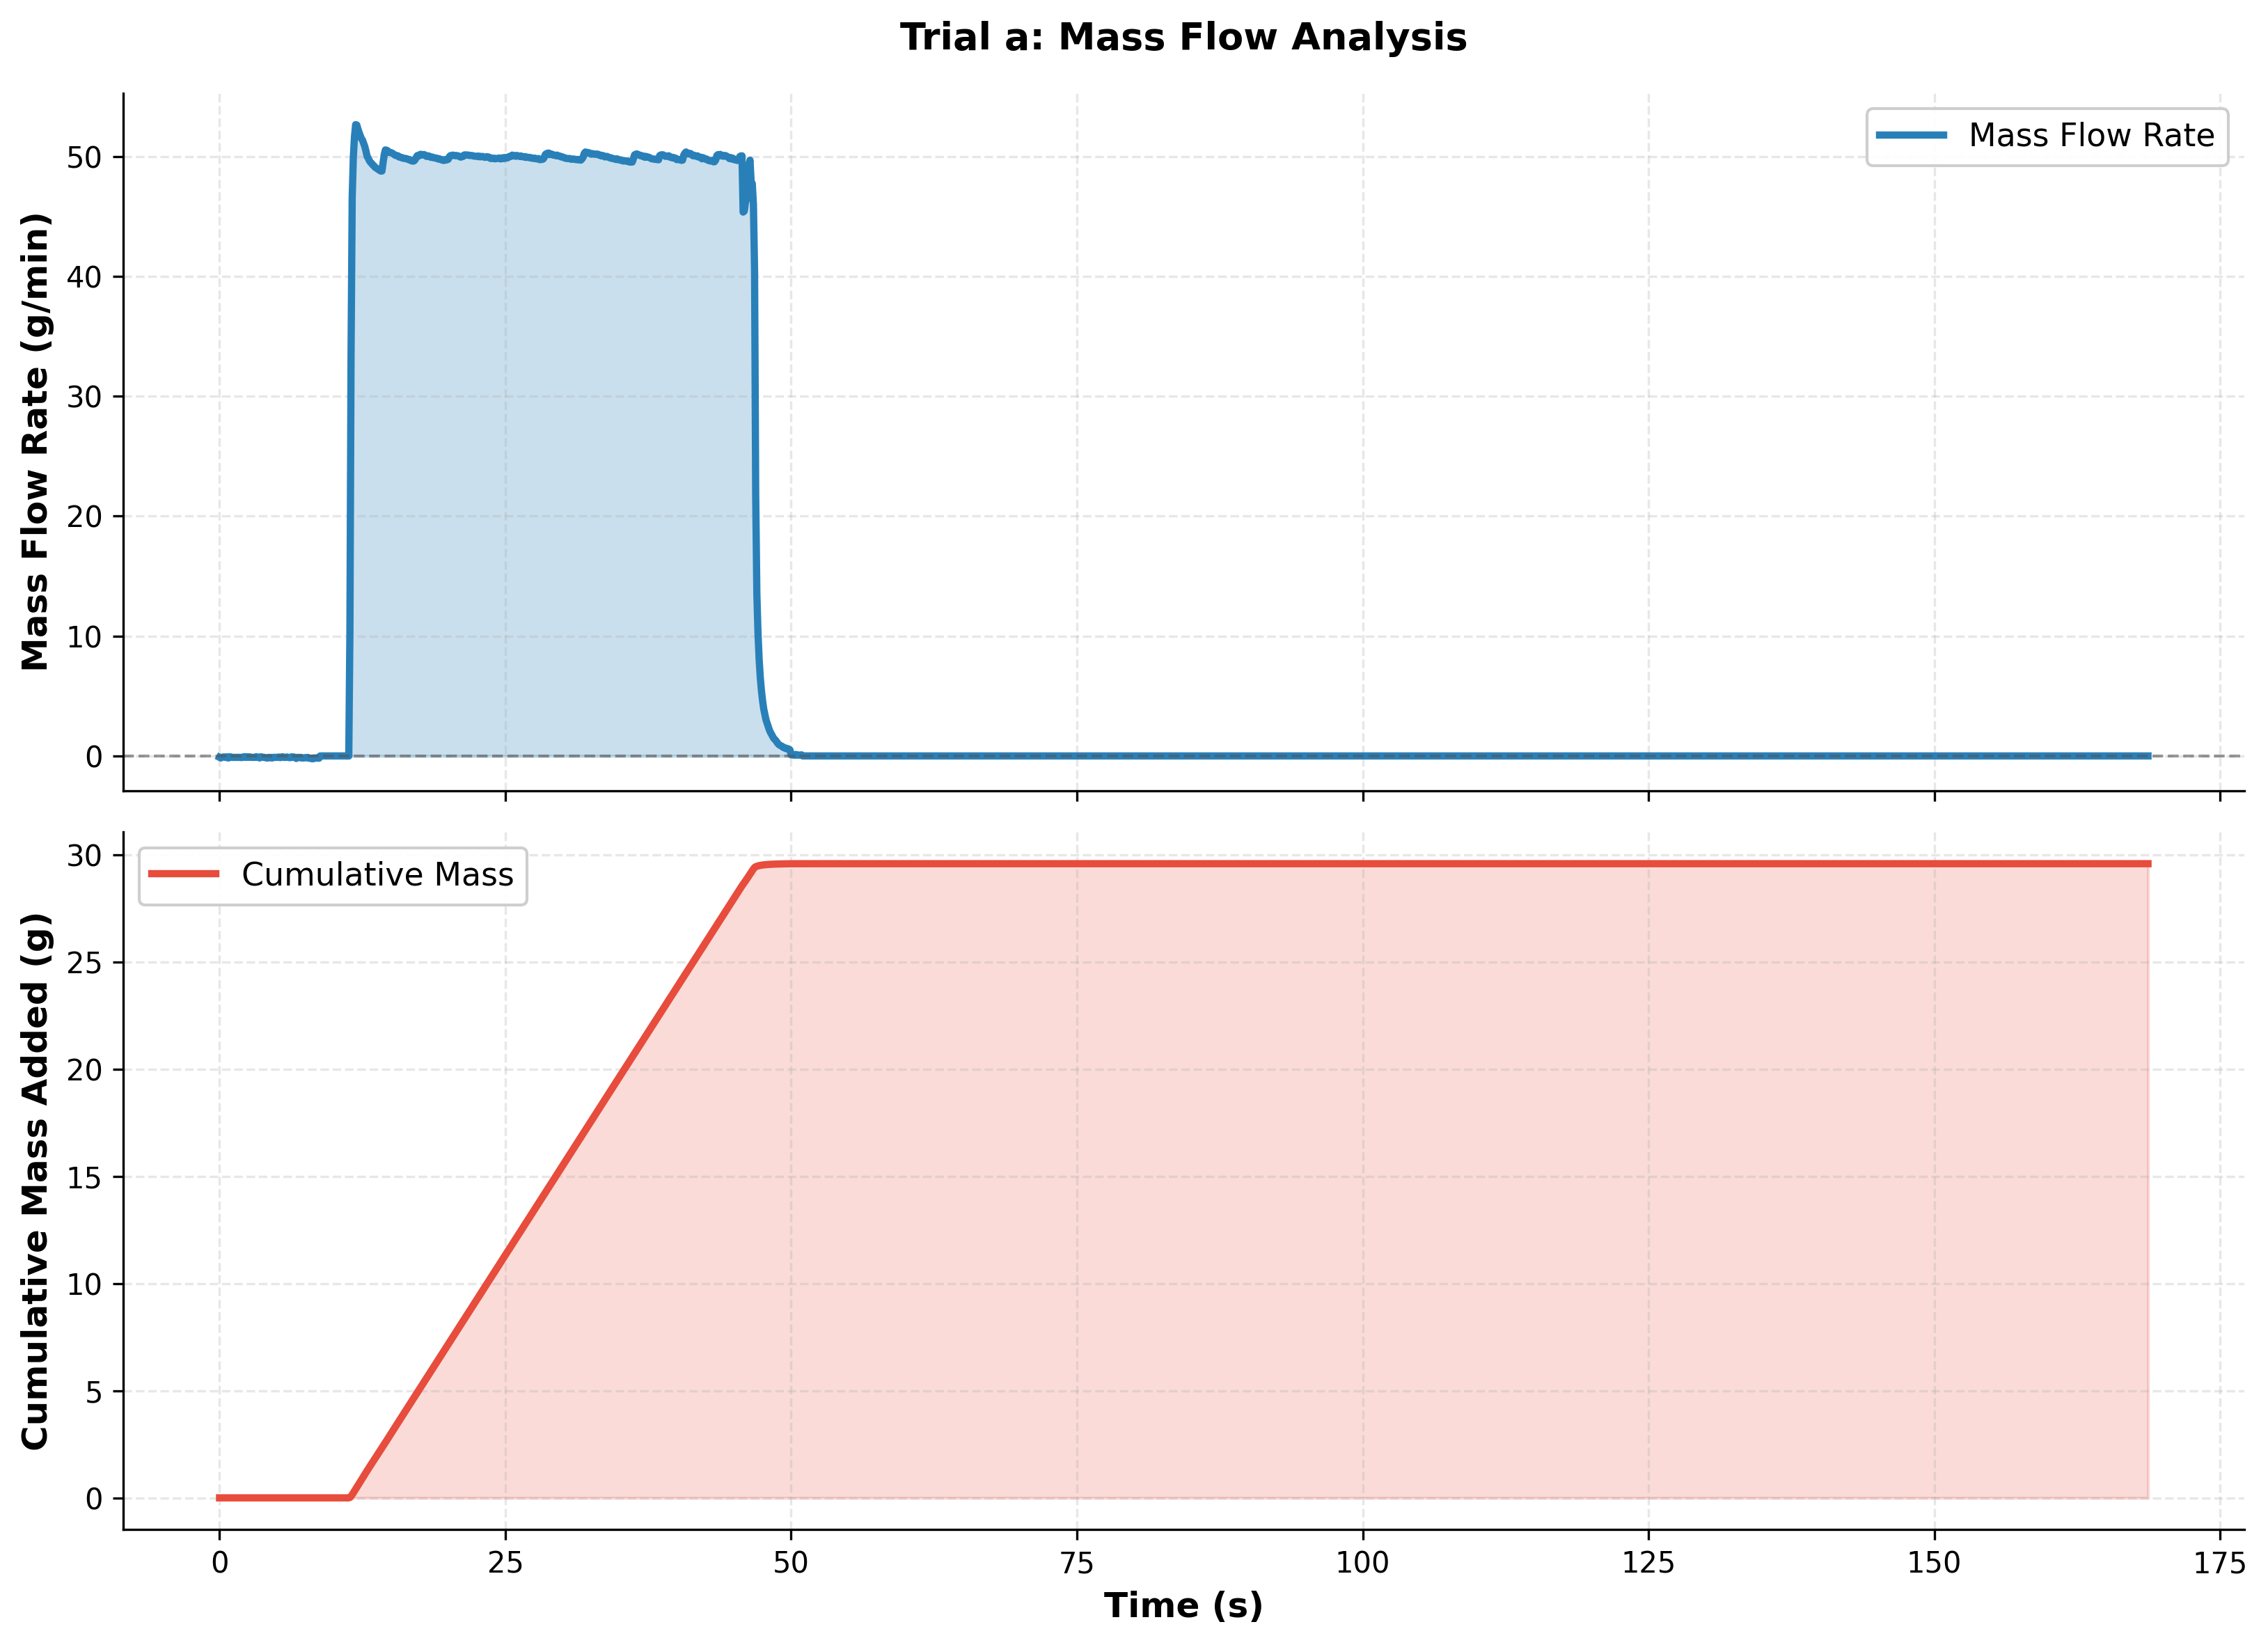
\includegraphics[width=0.85\textwidth]{graphs/part1_trial_a_mass_flow.png}
\caption{Example (Trial A): mass-flow vs.\ time and cumulative added mass. Similar curves were obtained for trials B--D (See Appendix B.1).}
\label{fig:part1_massflow}
\end{figure}

\subsection*{Part 2 — Heat Loss at Steady State}
\paragraph{Heat loss from input power.} For each trial, a linear fit was applied to the cumulative heater energy $Q(t)$ over a 5 minute steady state window (temperature plateau $\pm 0.5$ K). The fitted slope yielded the steady state heat loss rate $\dot{Q}_{\text{total}}$ used in Table~\ref{tab:part2}. Uncertainties were propagated from the heater power supply accuracy ($\pm 0.07$ kW) and temperature sensor resolution ($\pm 0.1$ K), derived from the precision of the raw data collected ($0.1$s and $0.1$ kJ). A representative energy-vs-time fit is shown in Fig. \ref{fig:part2_energyfit}.

\begin{figure}[H]
\centering
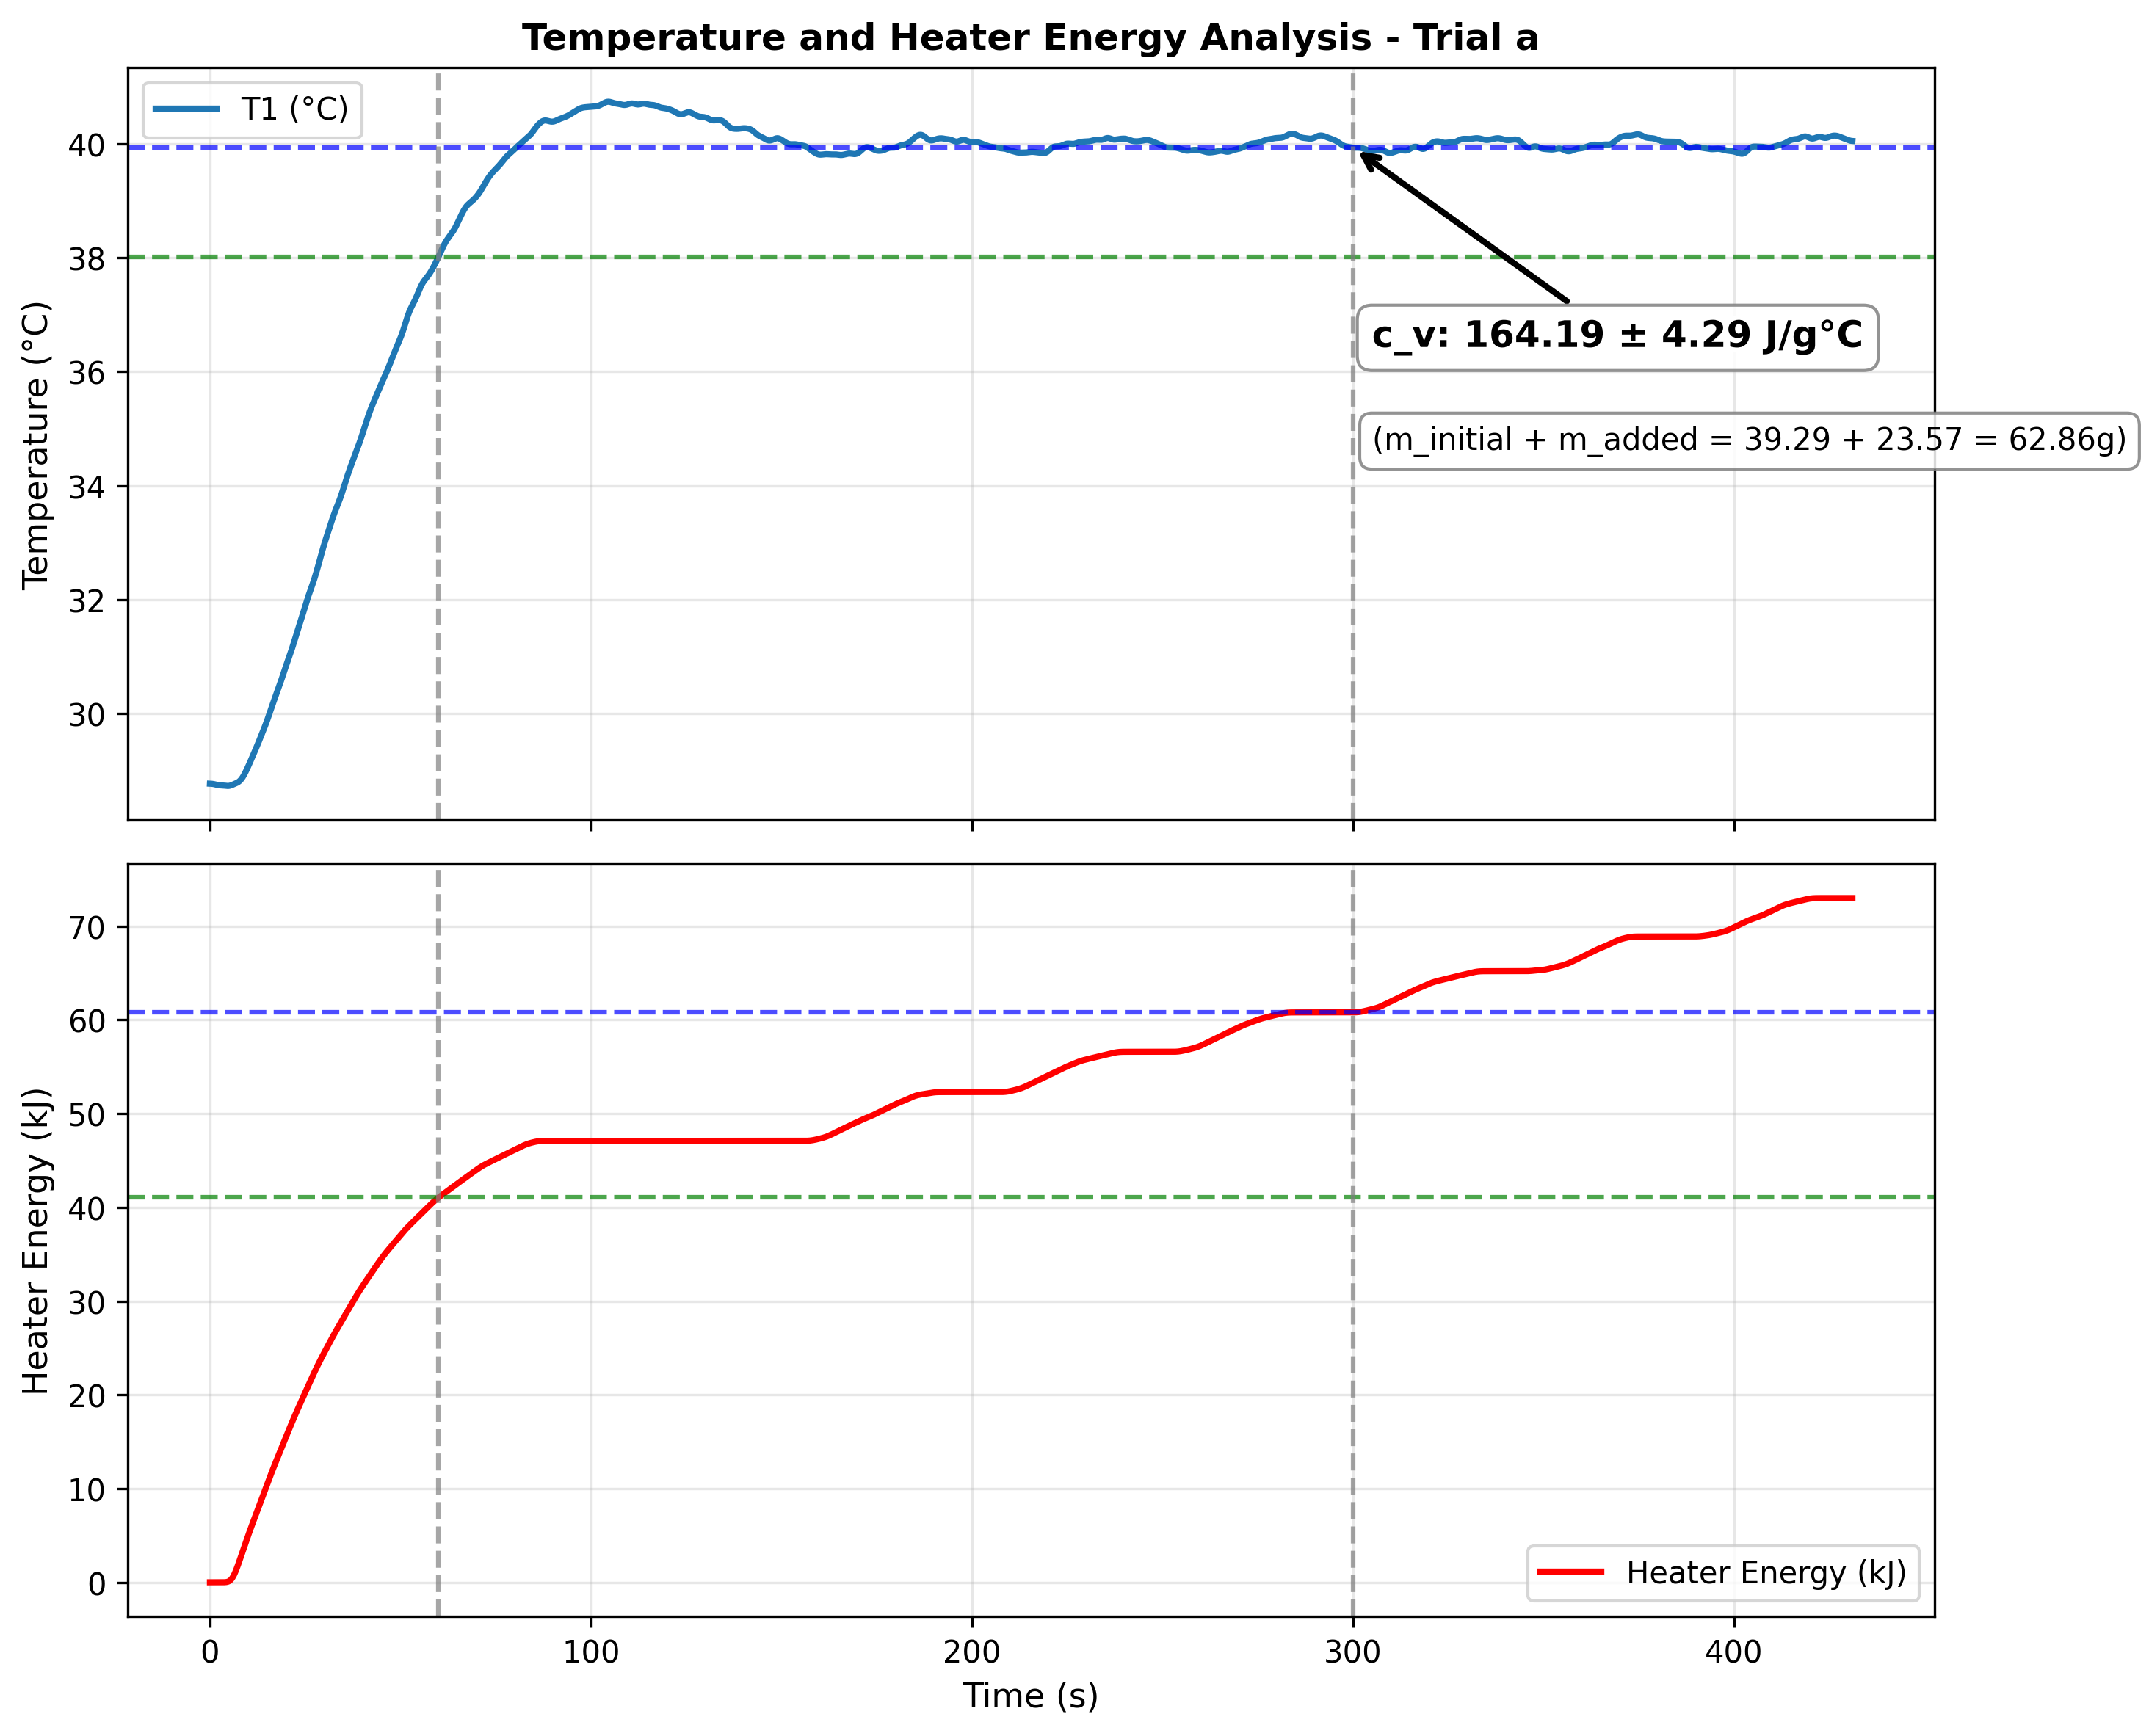
\includegraphics[width=0.85\textwidth]{graphs/part2_trial_a_temp_heater_energy.png}
\caption{Example (Trial A): heater energy (left, red) and tank temperature (right, blue) vs.\ time; shaded region marks the 5-min steady state window used for linear fit.}
\label{fig:part2_energyfit}
\end{figure}

\paragraph{Heat loss from walls and plates.} The acrylic wall heat conduction was calculated using the cylindrical conduction equation $\dot{Q} = \frac{2k\pi L\Delta T}{\ln(r_2/r_1)}$~\cite{che260_manual}, where thermal conductivity $k = 0.185$ W/(m·K) (acrylic), cylinder height $L = 0.286$ m, outer radius $r_2 = 50.8$ mm, and inner radius $r_1 = 41.3$ mm (after subtracting 9.525 mm wall thickness). The temperature difference $\Delta T = T_{\text{gas,ss}} - T_{\text{ambient}}$ was taken from measured steady state gas temperature and the recorded ambient temperature of 23.9 \textdegree C. Uncertainties in $k$, geometry, and $\Delta T$ were propagated via linear uncertainty analysis. The residual loss through the aluminum plates was calculated as $\dot{Q}_{\text{plates}} = \dot{Q}_{\text{total}} - \dot{Q}_{\text{acrylic}}$. The heat loss breakdown (Fig. \ref{fig:part2_breakdown}) shows that plates accounted for 85–87\% of total losses across all trials.

\begin{figure}[H]
\centering
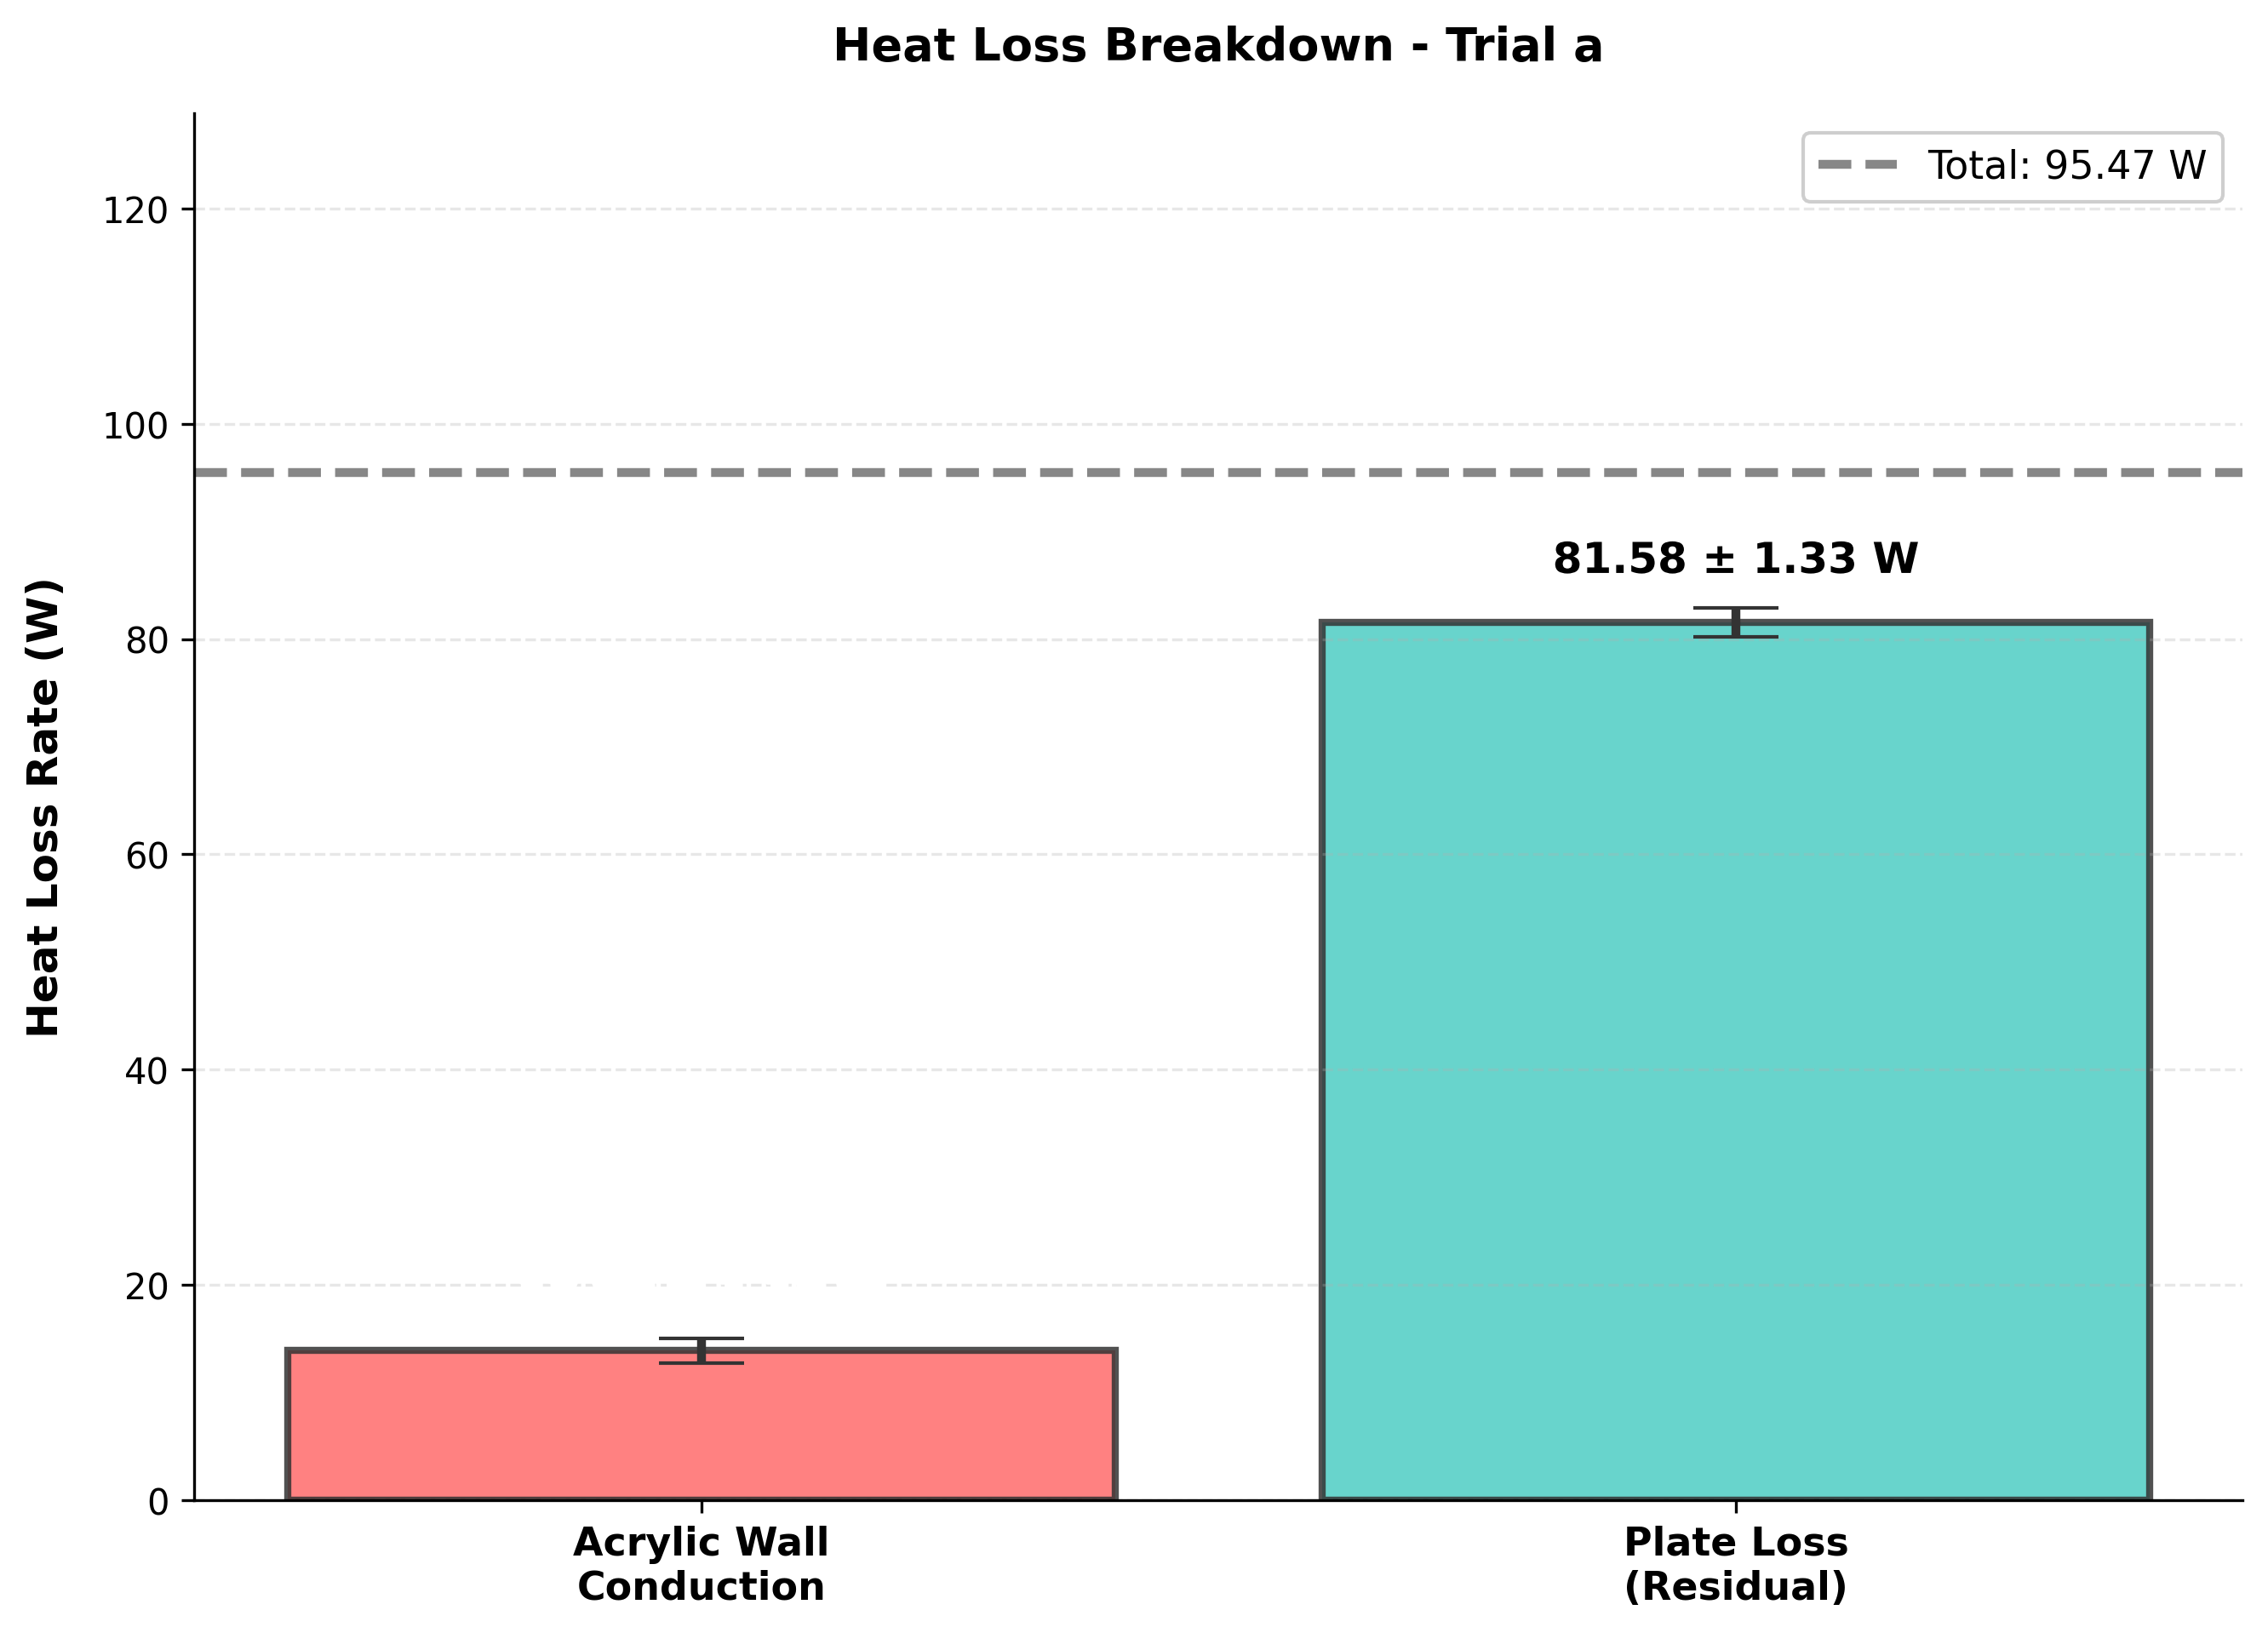
\includegraphics[width=0.85\textwidth]{graphs/part2_trial_a_loss_breakdown.png}
\caption{Example (Trial A): breakdown of steady state heat loss into acrylic wall conduction and aluminum plate residual losses.}
\label{fig:part2_breakdown}
\end{figure}

\begin{table}[H]\centering
\begin{tabular}{@{}lccccc@{}}
\toprule
Trial & $T_{\text{ss}}$ (\si{\celsius}) & $\dot Q_{\text{total}}$ (W) & $\dot Q_{\text{acrylic}}$ (W) & $\dot Q_{\text{plates}}$ (W) \\
\midrule
A & 40.0 & $95 \pm 1$ & $14 \pm 1$ & $82 \pm 1$ \\
B & 40.0 & $119 \pm 1$ & $13 \pm 1$ & $106 \pm 1$ \\
C & 59.2 & $210 \pm 0.2$ & $32 \pm 3$ & $178 \pm 3$ \\
D & 59.3 & $240 \pm 0.2$ & $29 \pm 2$ & $212 \pm 2$ \\
\bottomrule
\end{tabular}
\caption{Part 2 steady state summary (per trial).}
\label{tab:part2}
\end{table}

Heat loss increased from 95 W (Trial A) to 240 W (Trial D) as the setpoint temperature rose from 40 to 59 \textdegree C, confirming temperature-dependent loss mechanisms (convection and radiation to surroundings). The acrylic wall conducted 14–32 W, accounting for only 13–15\% of total loss; the remaining 85–87\% was lost through the aluminum plates, indicating that the plate conduction dominated. The linear fit of the heat loss rate and agreement between repeated trials validates that heat loss remains constant during the steady state plateau. Uncertainties ($\pm 0.2$ to $\pm 1$ W) were dominated by the heater power supply accuracy and temperature sensor noise.

\paragraph{Constant-volume specific heat $c_v$.} A heating segment of duration 24 s was selected in each trial, spanning the linear section of the rise from the initial temperature to near steady state (temperature increase of 3.4–8.6 K). 
Heater energy was integrated over the 24 s, and the steady state heat loss rate $\dot{Q}_{\text{total}}$ was used to estimate the net energy retained: $Q_{\text{net}} = Q_{\text{in}} - \dot{Q}_{\text{total}} \times \Delta t$. 
The specific heat was then calculated from $c_v = Q_{\text{net}} / (m \cdot \Delta T)$ \cite{che260_manual}, where $m$ was the mass of air in the tank from Part 1 and $\Delta T$ was the temperature rise over the 24 s. Uncertainties were propagated from all contributing measurements using the method of partial derivatives.


\begin{table}[H]\centering
\begin{tabular}{@{}lcccc@{}}
\toprule
Trial & $m$ (kg) & $\Delta T$ (K) & $Q_{\text{in}}-Q_{\text{loss}}$ (kJ) & $c_v$ $(\mathrm{kJ\,kg^{-1}\,K^{-1}})$ \\
\midrule
A & 0.0629 & 4.3 & 24.5 & $82 \pm 10$ \\
B & 0.0825 & 3.4 & 20.6 & $63 \pm 9$ \\
C & 0.0618 & 8.6 & 47.4 & $80 \pm 10$ \\
D & 0.0794 & 8.2 & 47.6 & $64 \pm 10$ \\
\bottomrule
\end{tabular}
\caption{$c_v$ estimates from heating segments.}
\label{tab:cv}
\end{table}

Measured $c_v$ values ranged from 63 to 82~$\mathrm{kJ/(kg \cdot K)}$ with relative uncertainties of $\pm 15\%$, which was approximately 90--100$\times$ the theoretical value of 0.718~$\mathrm{kJ/(kg \cdot K)}$ for ideal air. 
This reflects errors in the transient calculation. The heating window used (24 s) yielded small $\Delta T$ (3.4--8.6 K), which amplified relative measurement noise. The mass $m$ was computed via ideal gas law at fixed inlet conditions, which neglected possible unideal dynamic pressure-volume effects. The efficiency of the heater could also play a role in the $c_v$ values being very large because $Q_{\text{in}}$ measures the total electric energy supplied, not accounting for any losses. 
The internal consistency (smaller $c_v$ for trials B and D with larger $m$, larger $c_v$ for trials A and C with smaller $m$) indicates there's likely a systematic error. 

\subsection*{Part 3 — Propeller Work and Temperature Rise}

Fan propeller power was estimated using the similarity law: $P_2 = P_1 \cdot (\rho_2/\rho_1) \cdot (n_2/n_1)^3 \cdot (D_2/D_1)^5$~\cite{che260_manual}. It was calcualted with the values provided by the manufacturer ($P_1 = 0.7457$ W at $n_1 = 4200$ rpm and standard air density), and matching conditions ($n_2 = 4200$ rpm, $\rho_2/\rho_1 \approx 1$ at similar ambient conditions).
The rate of temperature rise due to work done by the propeller was estimated from $\dot{T} = P_2 / (m \cdot c_v)$, where $c_v$ was taken from the corresponding trial's Part 2 calculation. Results are summarized in Table \ref{tab:prop}.

\begin{table}[H]\centering
\begin{tabular}{@{}lcccc@{}}
\toprule
Trial & $n_2$ (rpm) & $P_2$ (W) & $m$ (kg) & $\dot T$ (\si{K\,s^{-1}}) \\
\midrule
A & 4200 & $0.74 \pm 0.07$ & 0.0629 & $(1.4 \pm 0.1) \times 10^{-4}$ \\
B & 4200 & $0.74 \pm 0.07$ & 0.0825 & $(1.4 \pm 0.1) \times 10^{-4}$ \\
C & 4200 & $0.74 \pm 0.07$ & 0.0618 & $(1.5 \pm 0.1) \times 10^{-4}$ \\
D & 4200 & $0.74 \pm 0.07$ & 0.0794 & $(1.5 \pm 0.1) \times 10^{-4}$ \\
\bottomrule
\end{tabular}
\caption{Propeller work and implied temperature rise rate.}
\label{tab:prop}
\end{table}

Propeller power was constant at $P_2 = 0.74 \pm 0.07$ W across all trials, corresponding to a temperature rise rate of only $\dot{T} = 1.4 \text{ to } 1.5 \times 10^{-4}$ K/s. 
This is negligible compared to the main heat input rate because $\dot{Q}_{\text{total}} \sim 100$ W would cause $\dot{T} \sim 10^{-2}$ K/s, confirming that the propeller work plays a small roll in the overall energy balance. The negligible fan input also justifies dropping the work term from the steady state energy balance equation, meaning $\dot{Q} \approx \dot{m} c_p \Delta T_{\text{surroundings}}$. 

\section*{Conclusion}
This experiment investigated the First Law of Thermodynamics in a closed, pressurized air tank by measuring heat loss, work input, and internal energy changes.
The behavior of the mass of air was accurately predicted by the ideal gas law, validating the measurement approach.
Steady state heat loss rates increased with temperature (from 95~W at 40~$^{\circ}$C to 242~W at 60~$^{\circ}$C), with with 85--87\% of losses through the aluminum plates and 13--15\% through the acrylic walls.
The calculated specific heat capacities ($c_v = 63$--$82~\mathrm{kJ/(kg \cdot K)}$) were significantly higher than theoretical values due to experimental limitations, including small temperature rises and ideal gas assumptions.
The propeller fan work was determined to be negligible ($\sim 0.7$ W) compared to heat loss, justifying its exclusion from the energy balance.


\begin{thebibliography}{9}
\bibitem{che260_manual}
CHE260 Course Notes, \textit{1st Law of Thermodynamics Laboratory Manual}. Toronto: University of Toronto, 2025.

\bibitem{che260_guidelines}
CHE260 Course Handout, \textit{Lab Report Guidelines}. Toronto: University of Toronto, 2025.
\end{thebibliography}

\newpage

\appendix

\section*{Appendix A: Sample Analysis Code}

The data analysis was automated using Python 3.13 with \texttt{numpy}, \texttt{pandas}, \texttt{scipy}, and \texttt{matplotlib}. Key functions include:

\subsection*{A.1 Heat Loss Decomposition}

\begin{verbatim}
def conduction_split(df_ss):
    L = 0.28575  # cylinder height (m)
    r2 = 0.0508  # outer radius (m)
    r1 = r2 - 0.009525  # inner radius
    k_acrylic = 0.185  # W/m·K
    T_gas = df_ss['T1(Deg C)'].mean()
    delta_T = T_gas - 22  # ambient
    Q_acrylic = (2*k_acrylic*np.pi*L*delta_T) / np.log(r2/r1)
    return Q_acrylic
\end{verbatim}

\subsection*{A.2 Uncertainty Propagation}

\begin{verbatim}
from uncertainties import ufloat
Q_in_uf = ufloat(24500, 200)  # J
Q_loss_uf = ufloat(2287, 150)  # J
m_uf = ufloat(0.06287, 0.00005)  # kg
dT_uf = ufloat(4.3, 0.05)  # K
c_v = (Q_in_uf - Q_loss_uf) / (m_uf * dT_uf)
\end{verbatim}

\subsection*{A.3 Text Rendering}

\begin{verbatim}
def _auto_text_color(color):
    r,g,b = mcolors.to_rgb(color)
    L = 0.2126*r + 0.7152*g + 0.0722*b
    return 'white' if L < 0.6 else 'black'
\end{verbatim}

\section*{Appendix B: Graphs for All Trials}

\subsection*{B.1 Mass Flow (Trials B, C, D)}

\begin{figure}[H]
\centering
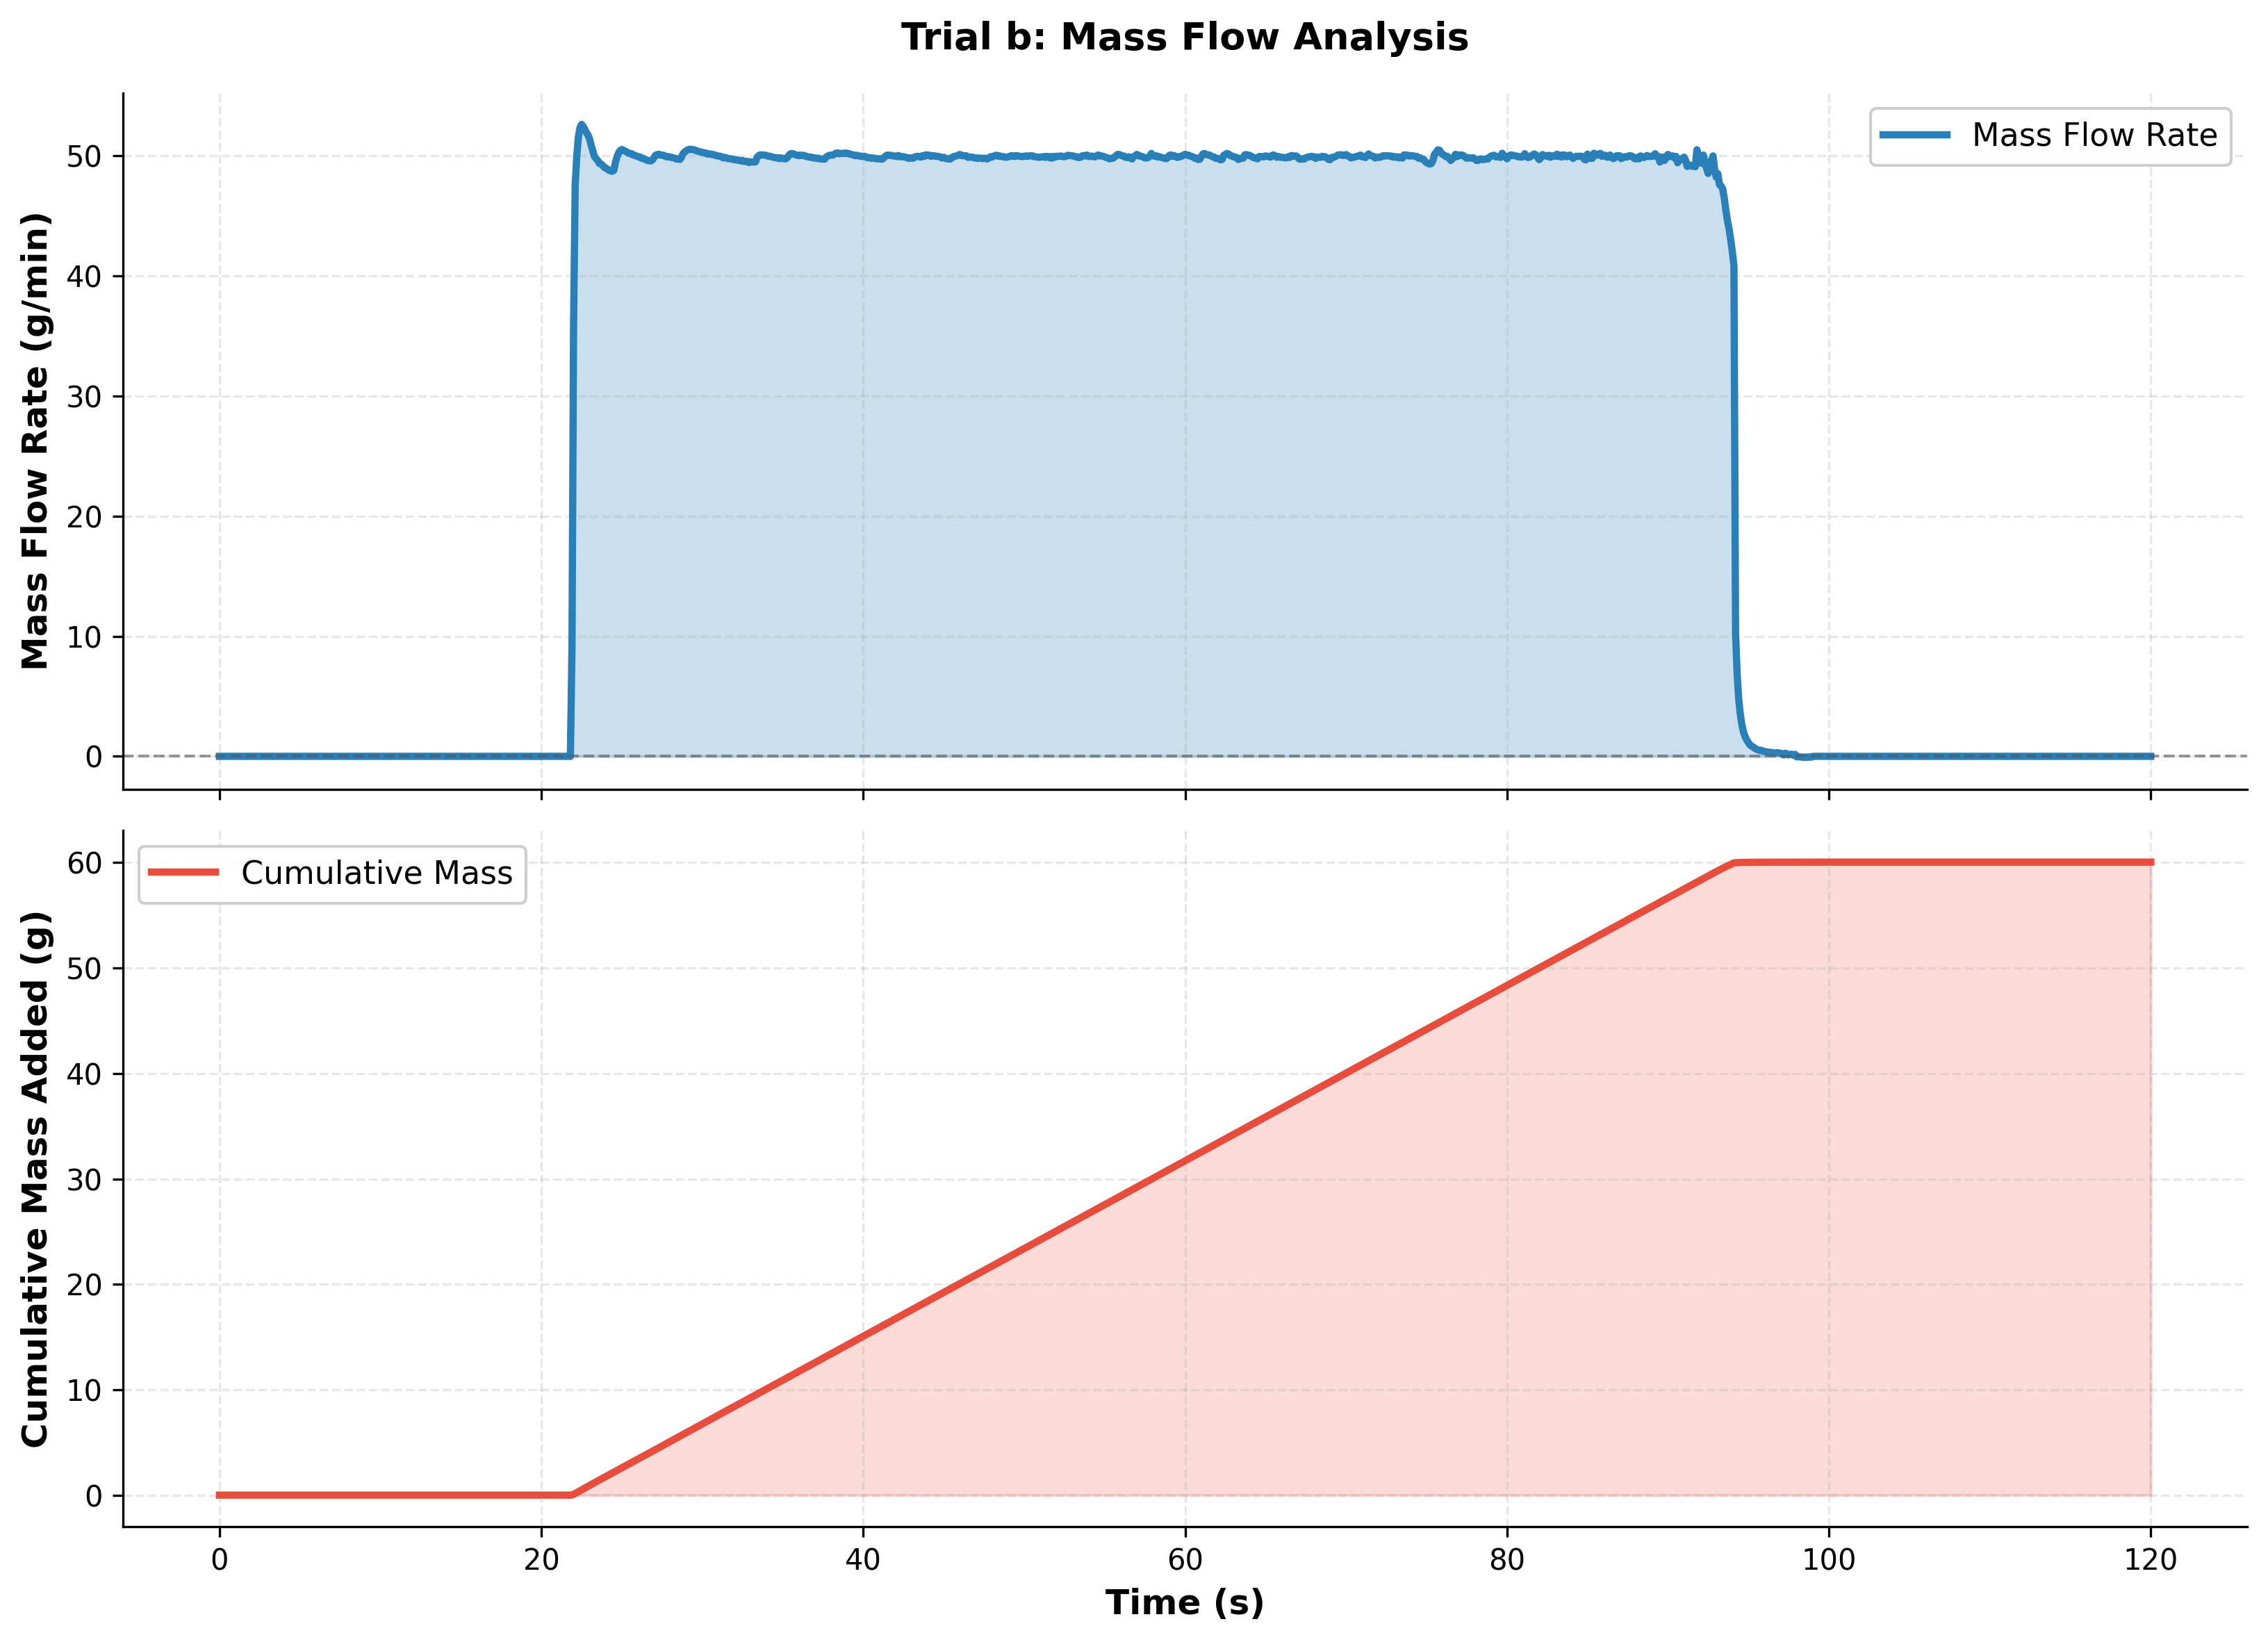
\includegraphics[width=0.85\textwidth]{graphs/part1_trial_b_mass_flow.png}
\caption{Mass flow rate: Trial B.}
\end{figure}

\begin{figure}[H]
\centering
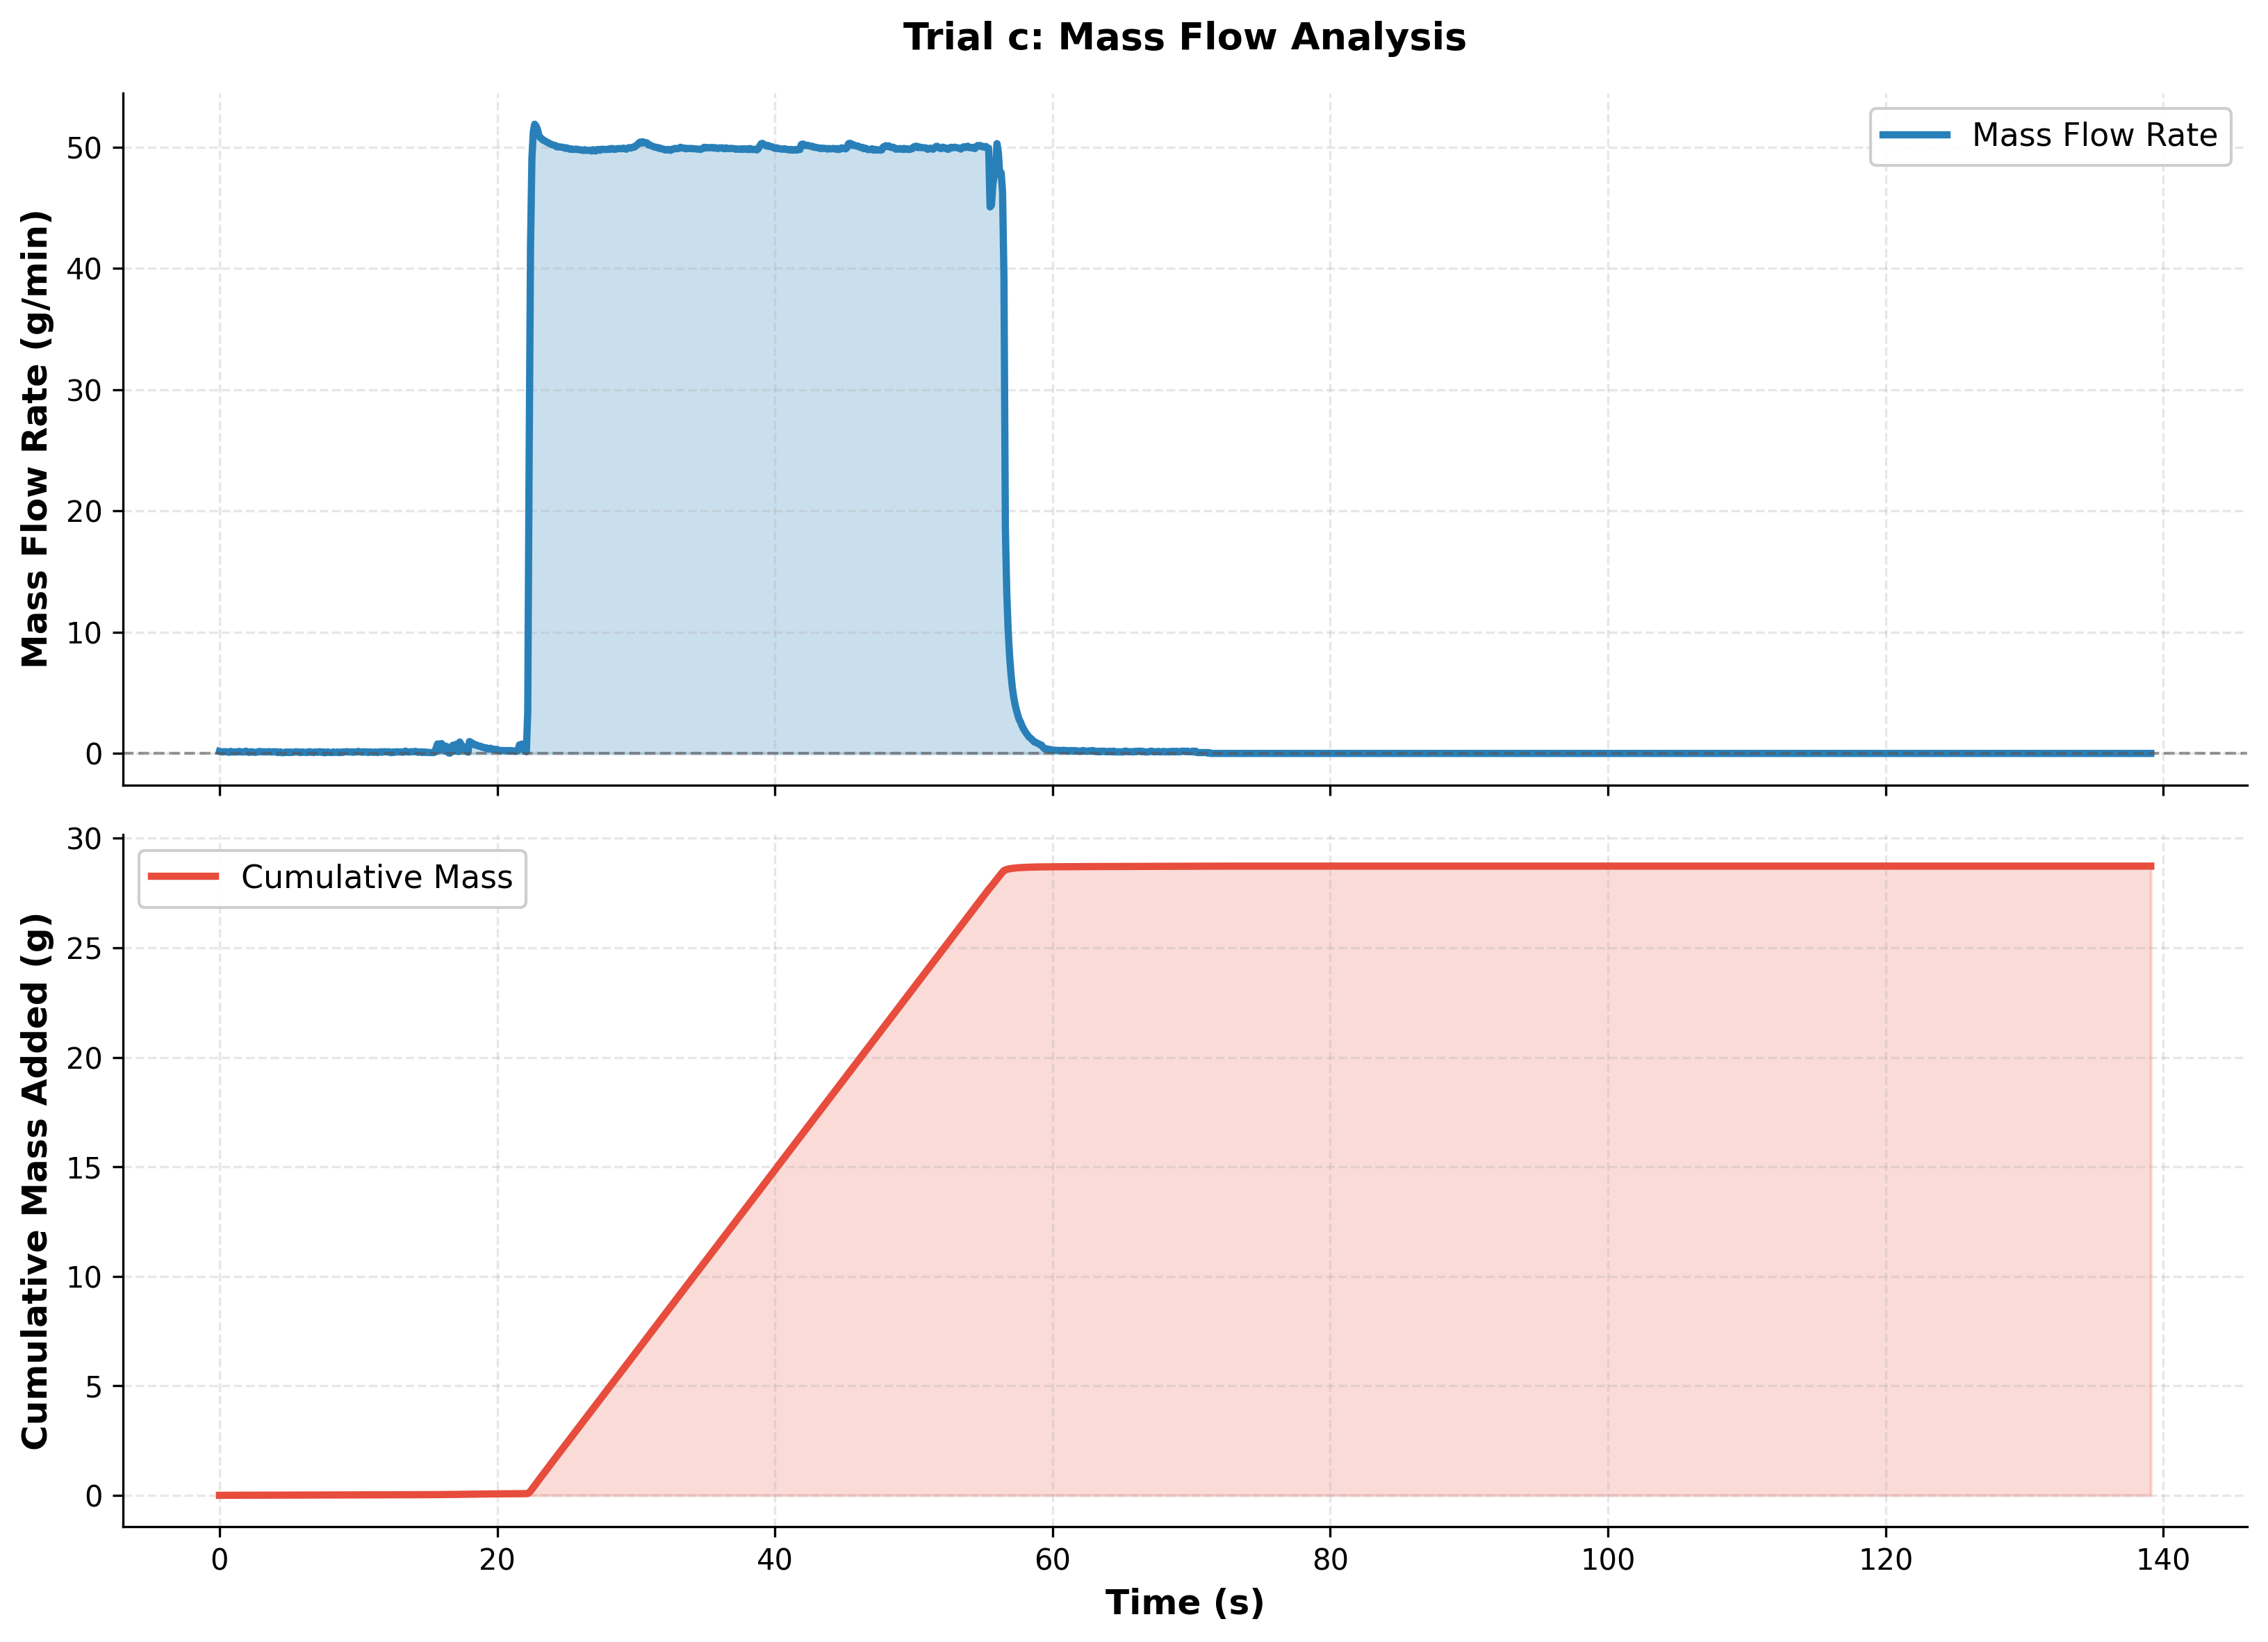
\includegraphics[width=0.85\textwidth]{graphs/part1_trial_c_mass_flow.png}
\caption{Mass flow rate: Trial C.}
\end{figure}

\begin{figure}[H]
\centering
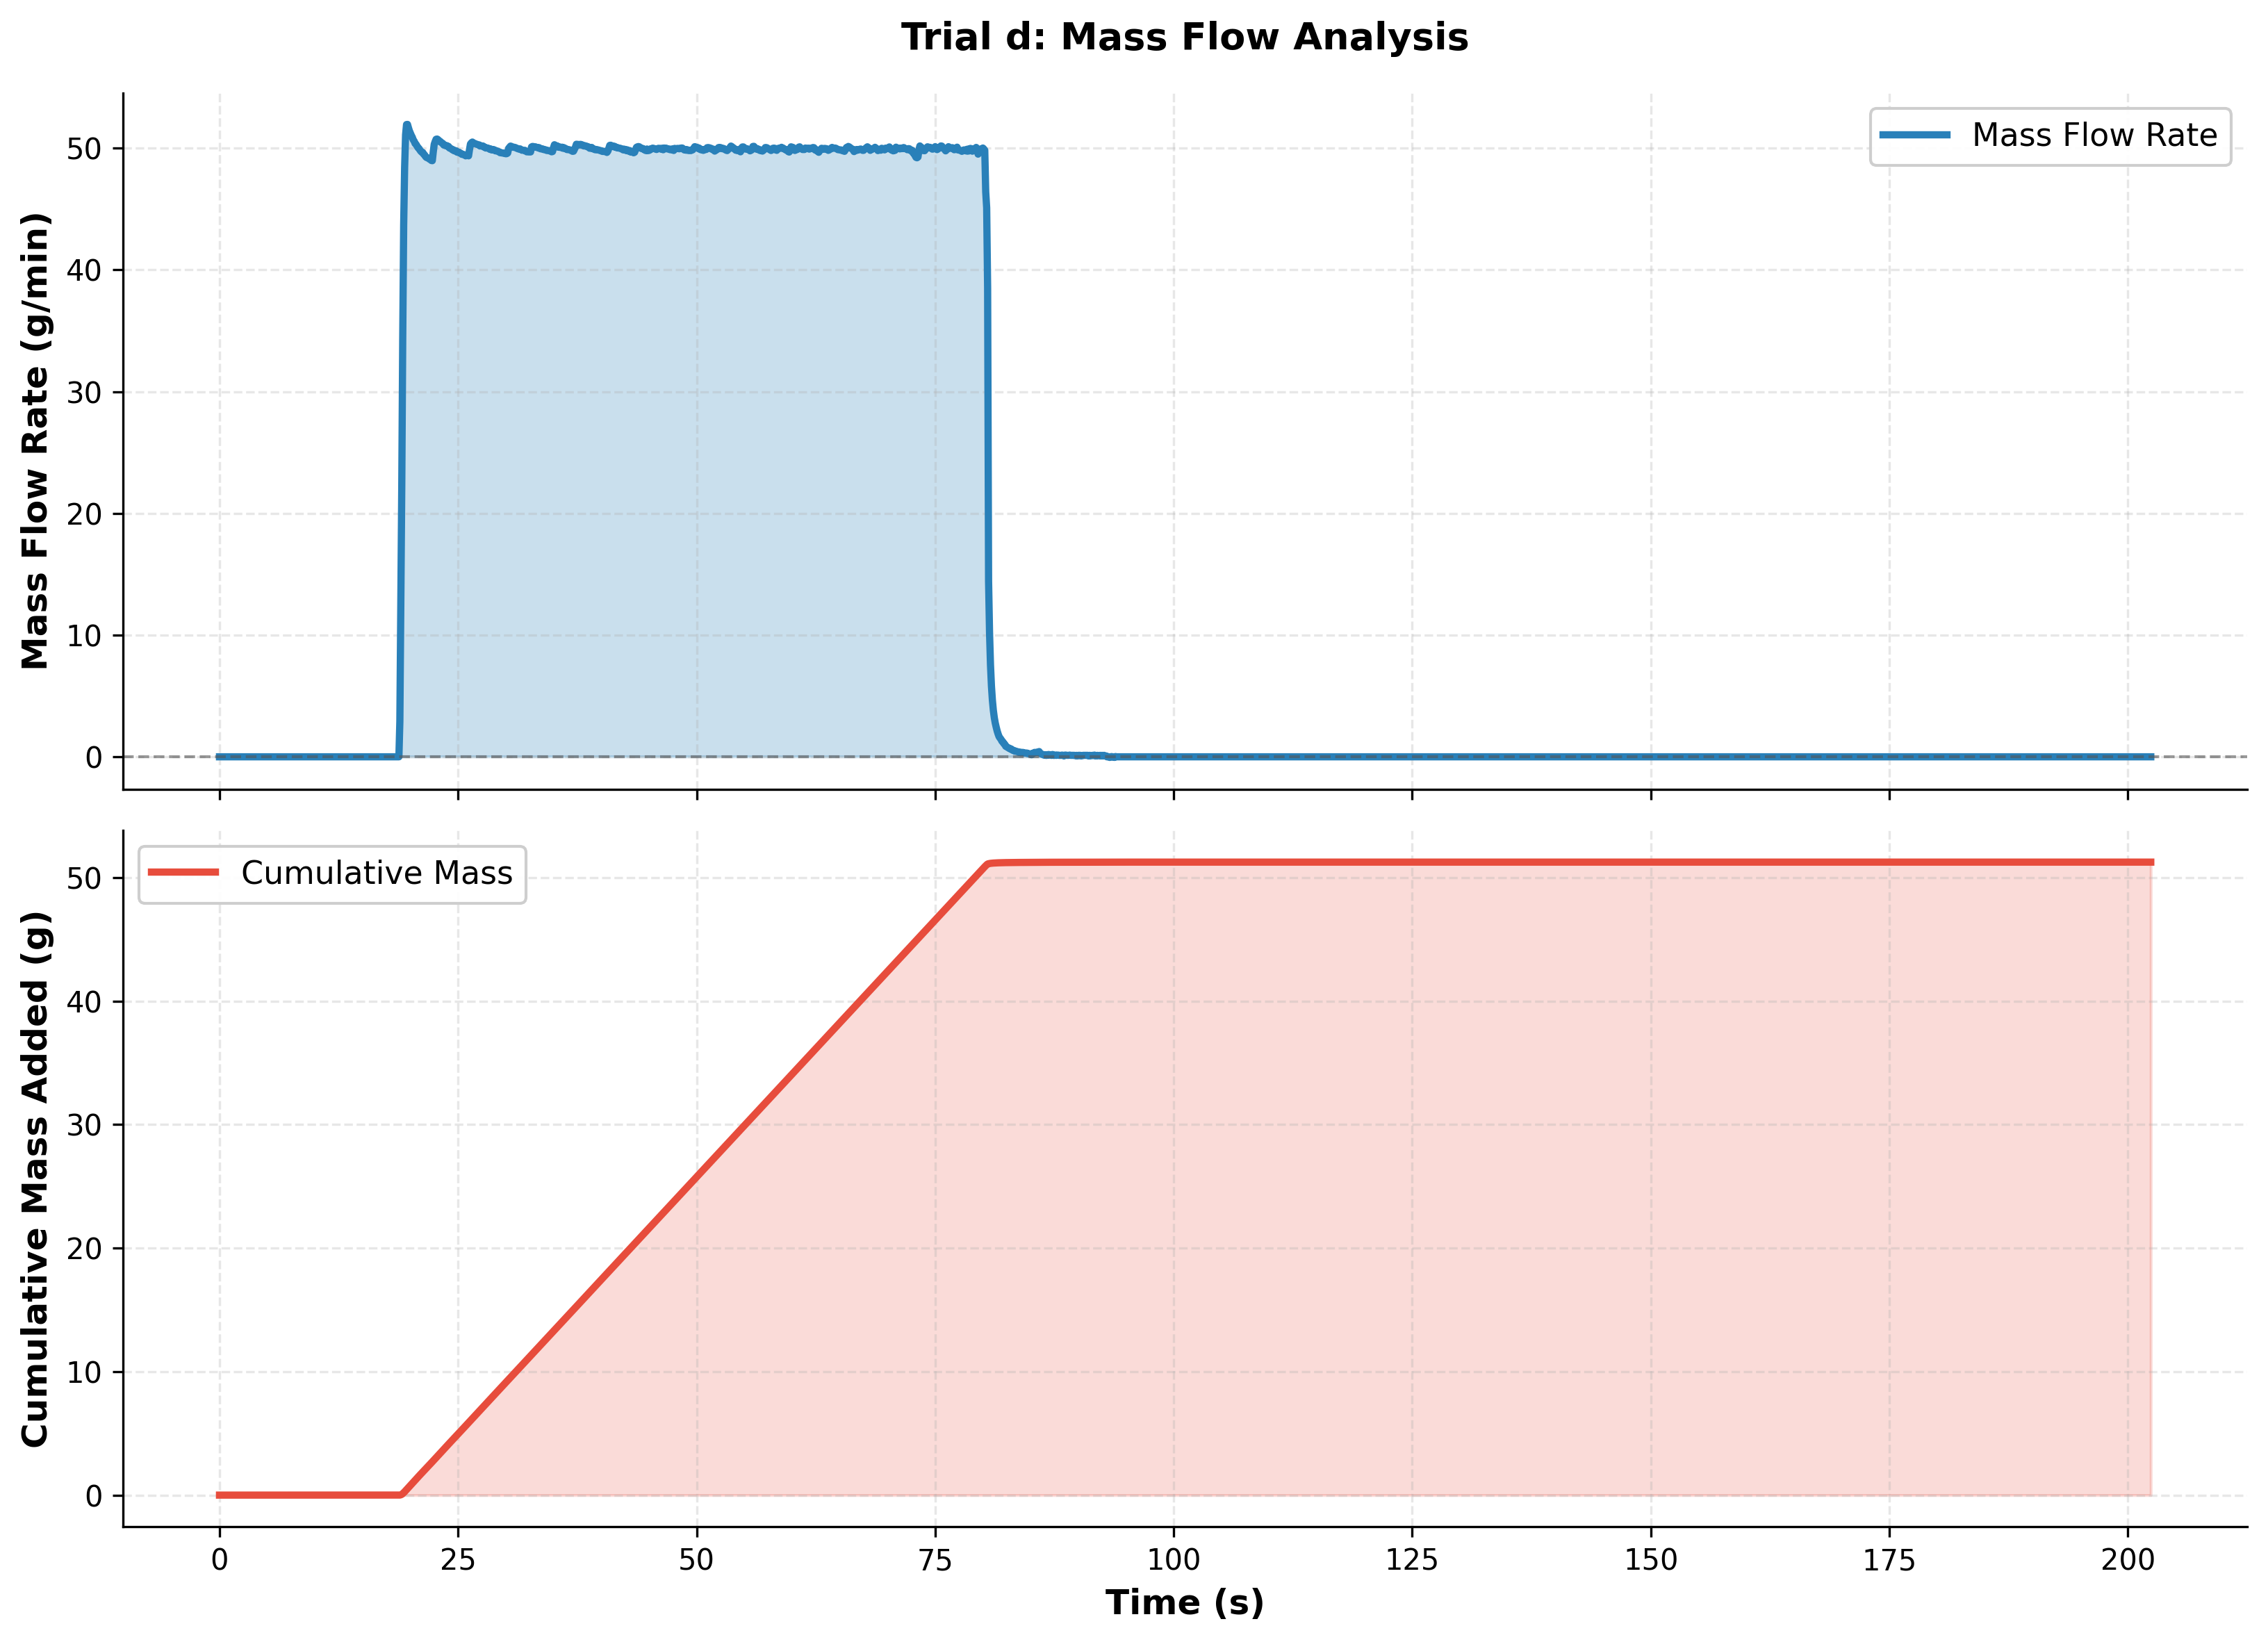
\includegraphics[width=0.85\textwidth]{graphs/part1_trial_d_mass_flow.png}
\caption{Mass flow rates: Trial D.}
\end{figure}

\subsection*{B.2 Temperature \& Energy (Trials B, C, D)}

\begin{figure}[H]
\centering
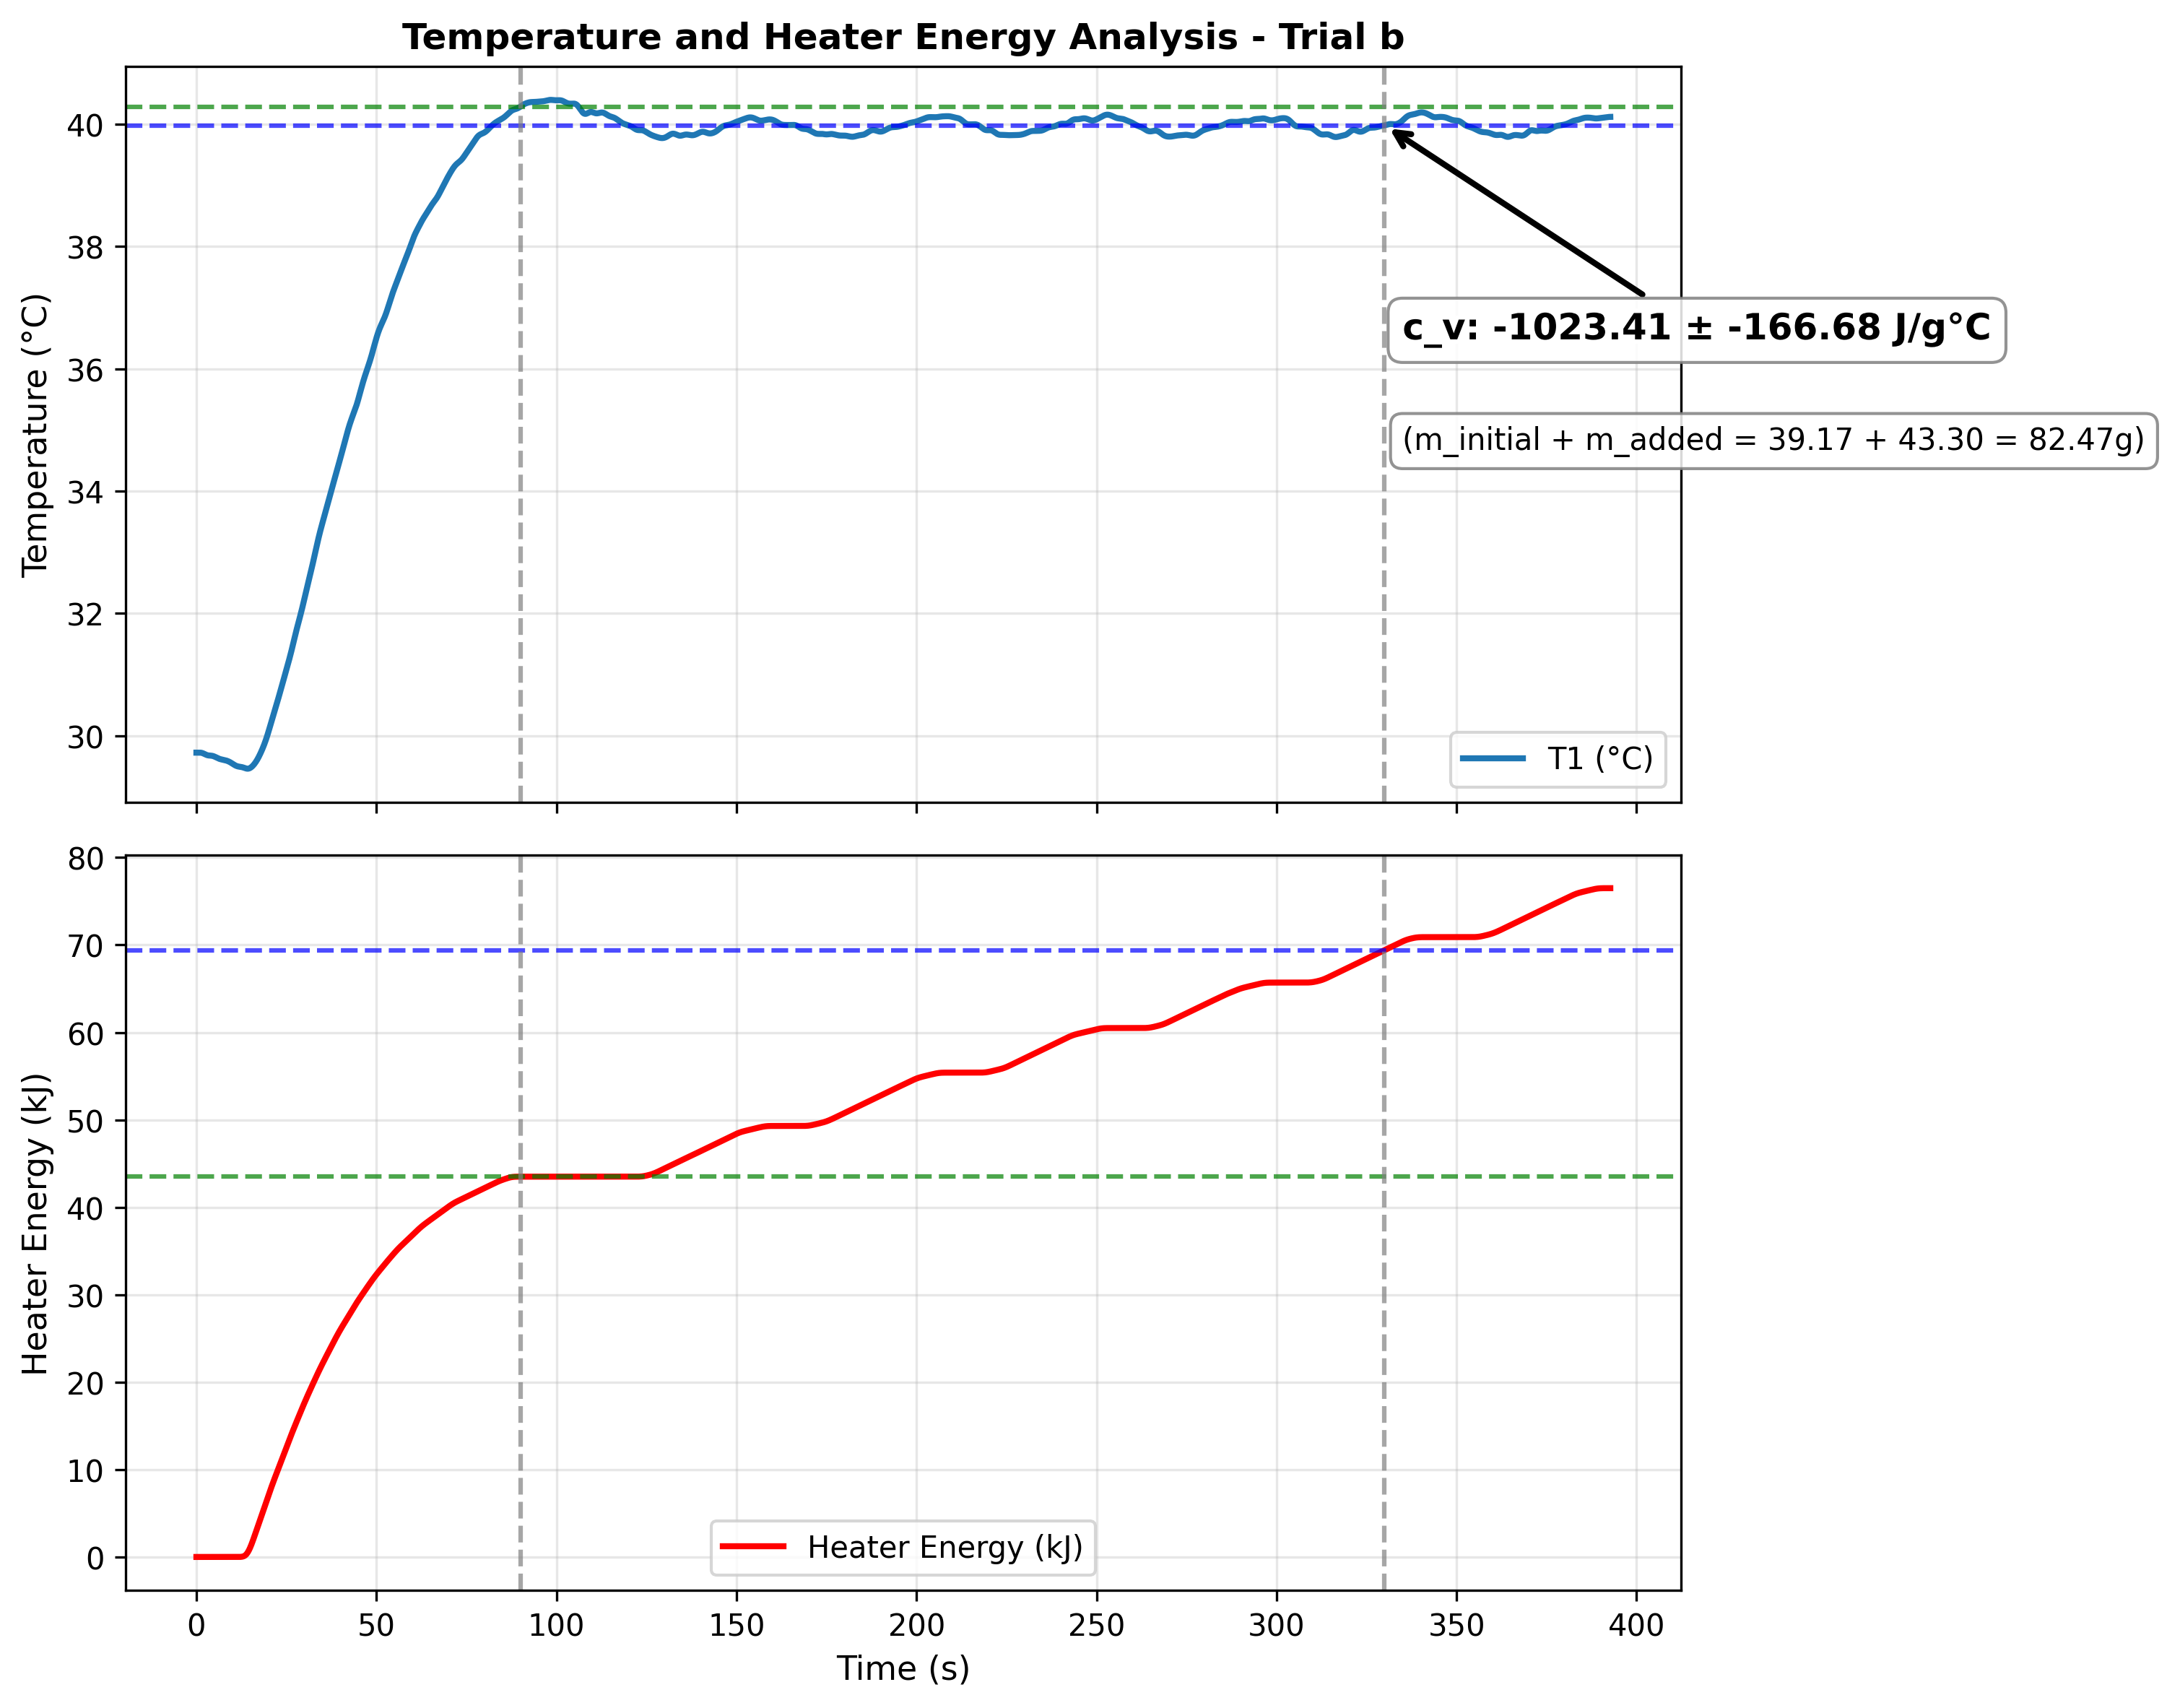
\includegraphics[width=0.85\textwidth]{graphs/part2_trial_b_temp_heater_energy.png}
\caption{Temperature and heater energy: Trial B.}
\end{figure}

\begin{figure}[H]
\centering
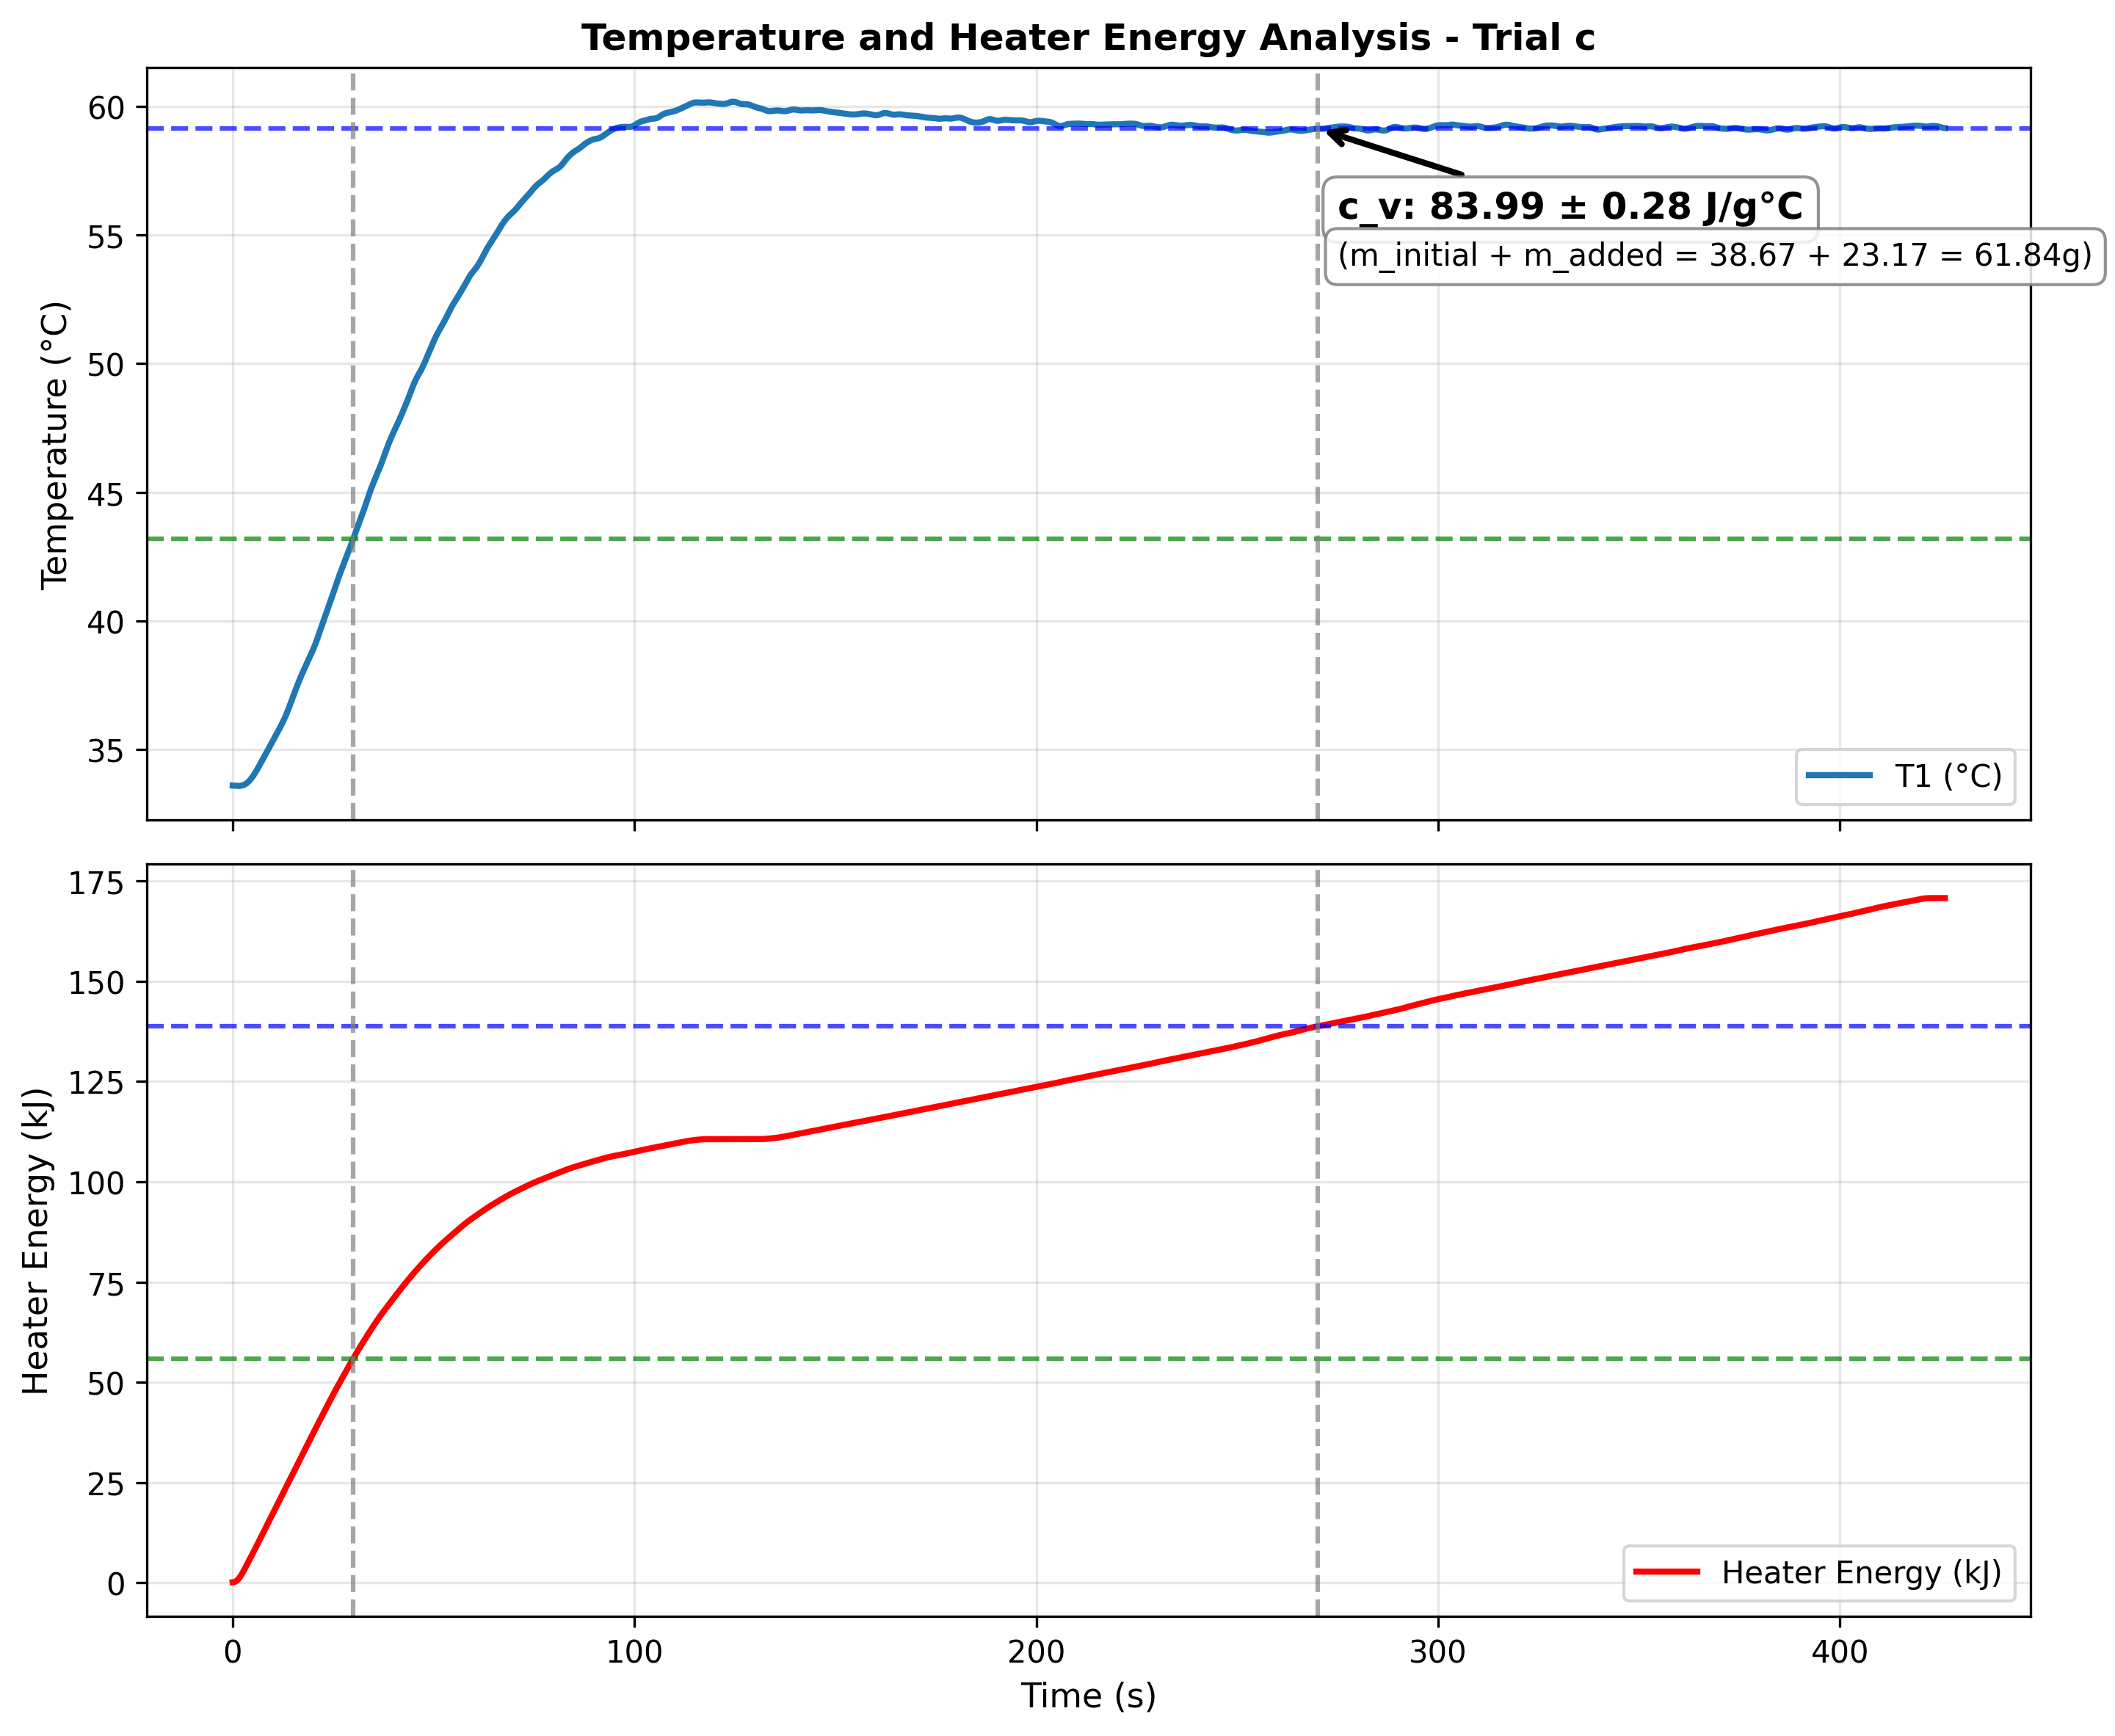
\includegraphics[width=0.85\textwidth]{graphs/part2_trial_c_temp_heater_energy.png}
\caption{Temperature and heater energy: Trial C.}
\end{figure}

\begin{figure}[H]
\centering
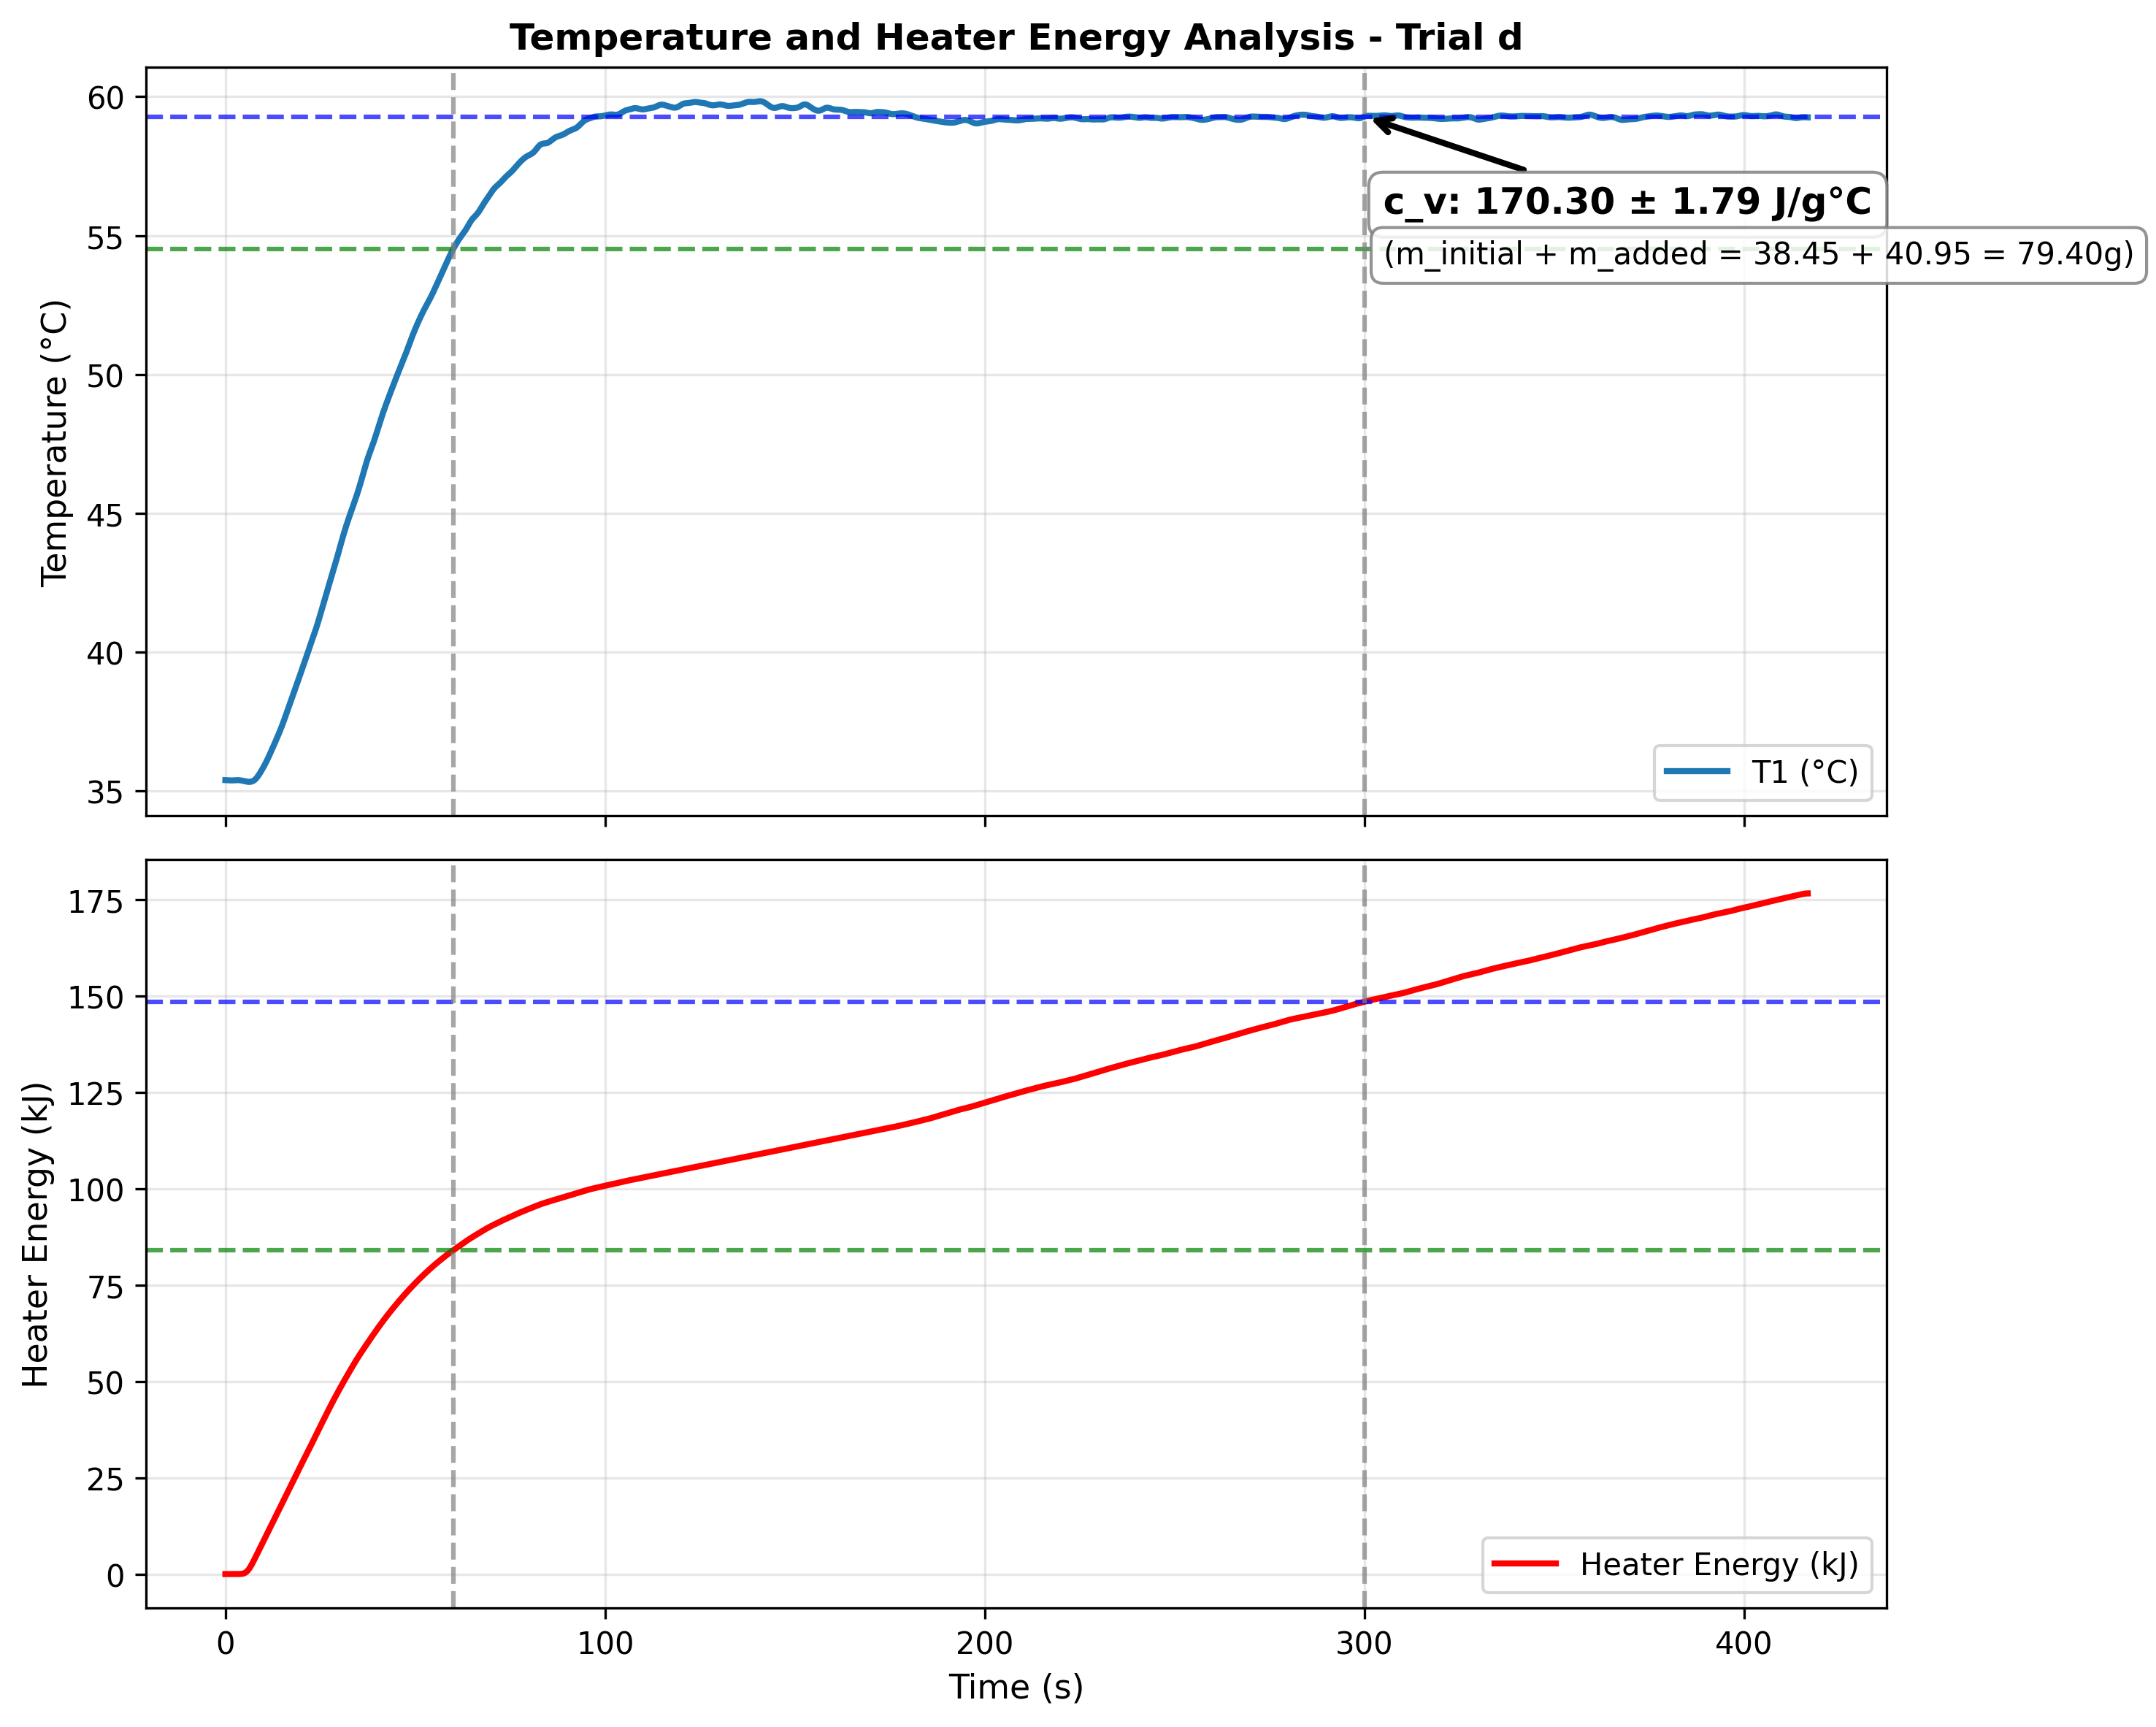
\includegraphics[width=0.85\textwidth]{graphs/part2_trial_d_temp_heater_energy.png}
\caption{Temperature and heater energy: Trial D.}
\end{figure}


\subsection*{B.3 steady state Maintenance (Trials B, C, D)}

\begin{figure}[H]
\centering
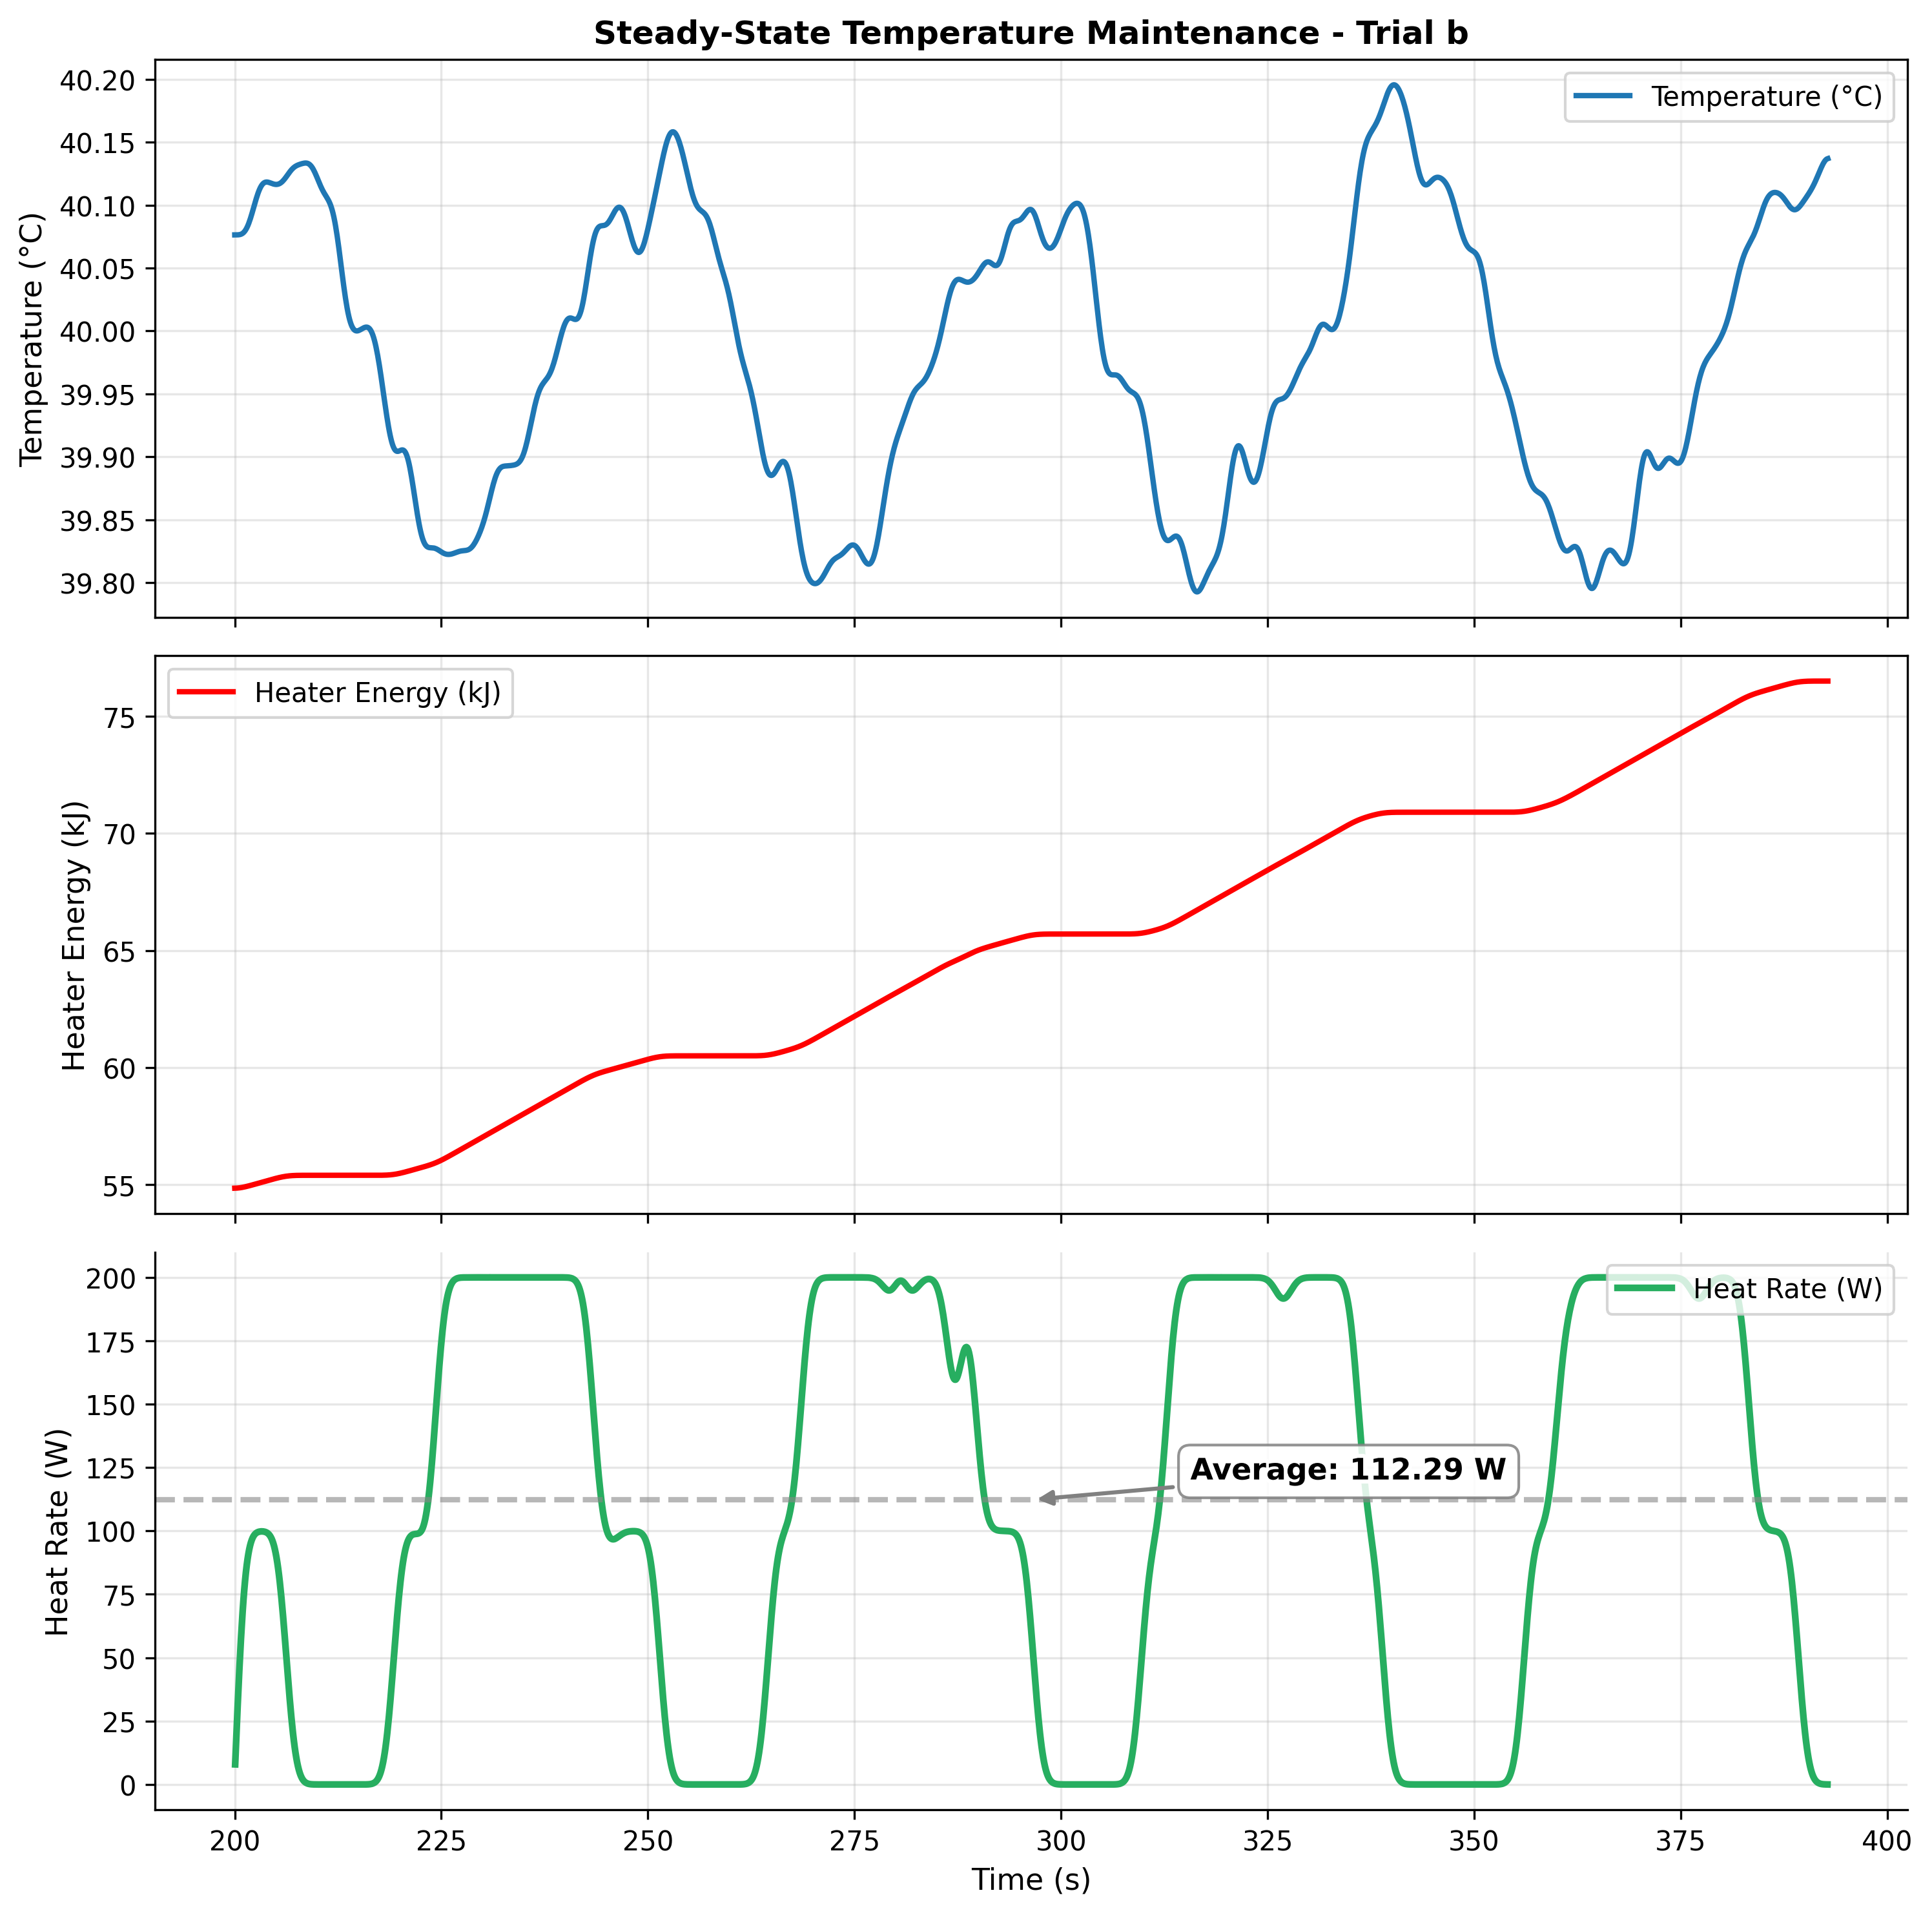
\includegraphics[width=0.85\textwidth]{graphs/part2_trial_b_heater_maintenance.png}
\caption{steady state plateau: Trial B.}
\end{figure}

\begin{figure}[H]
\centering
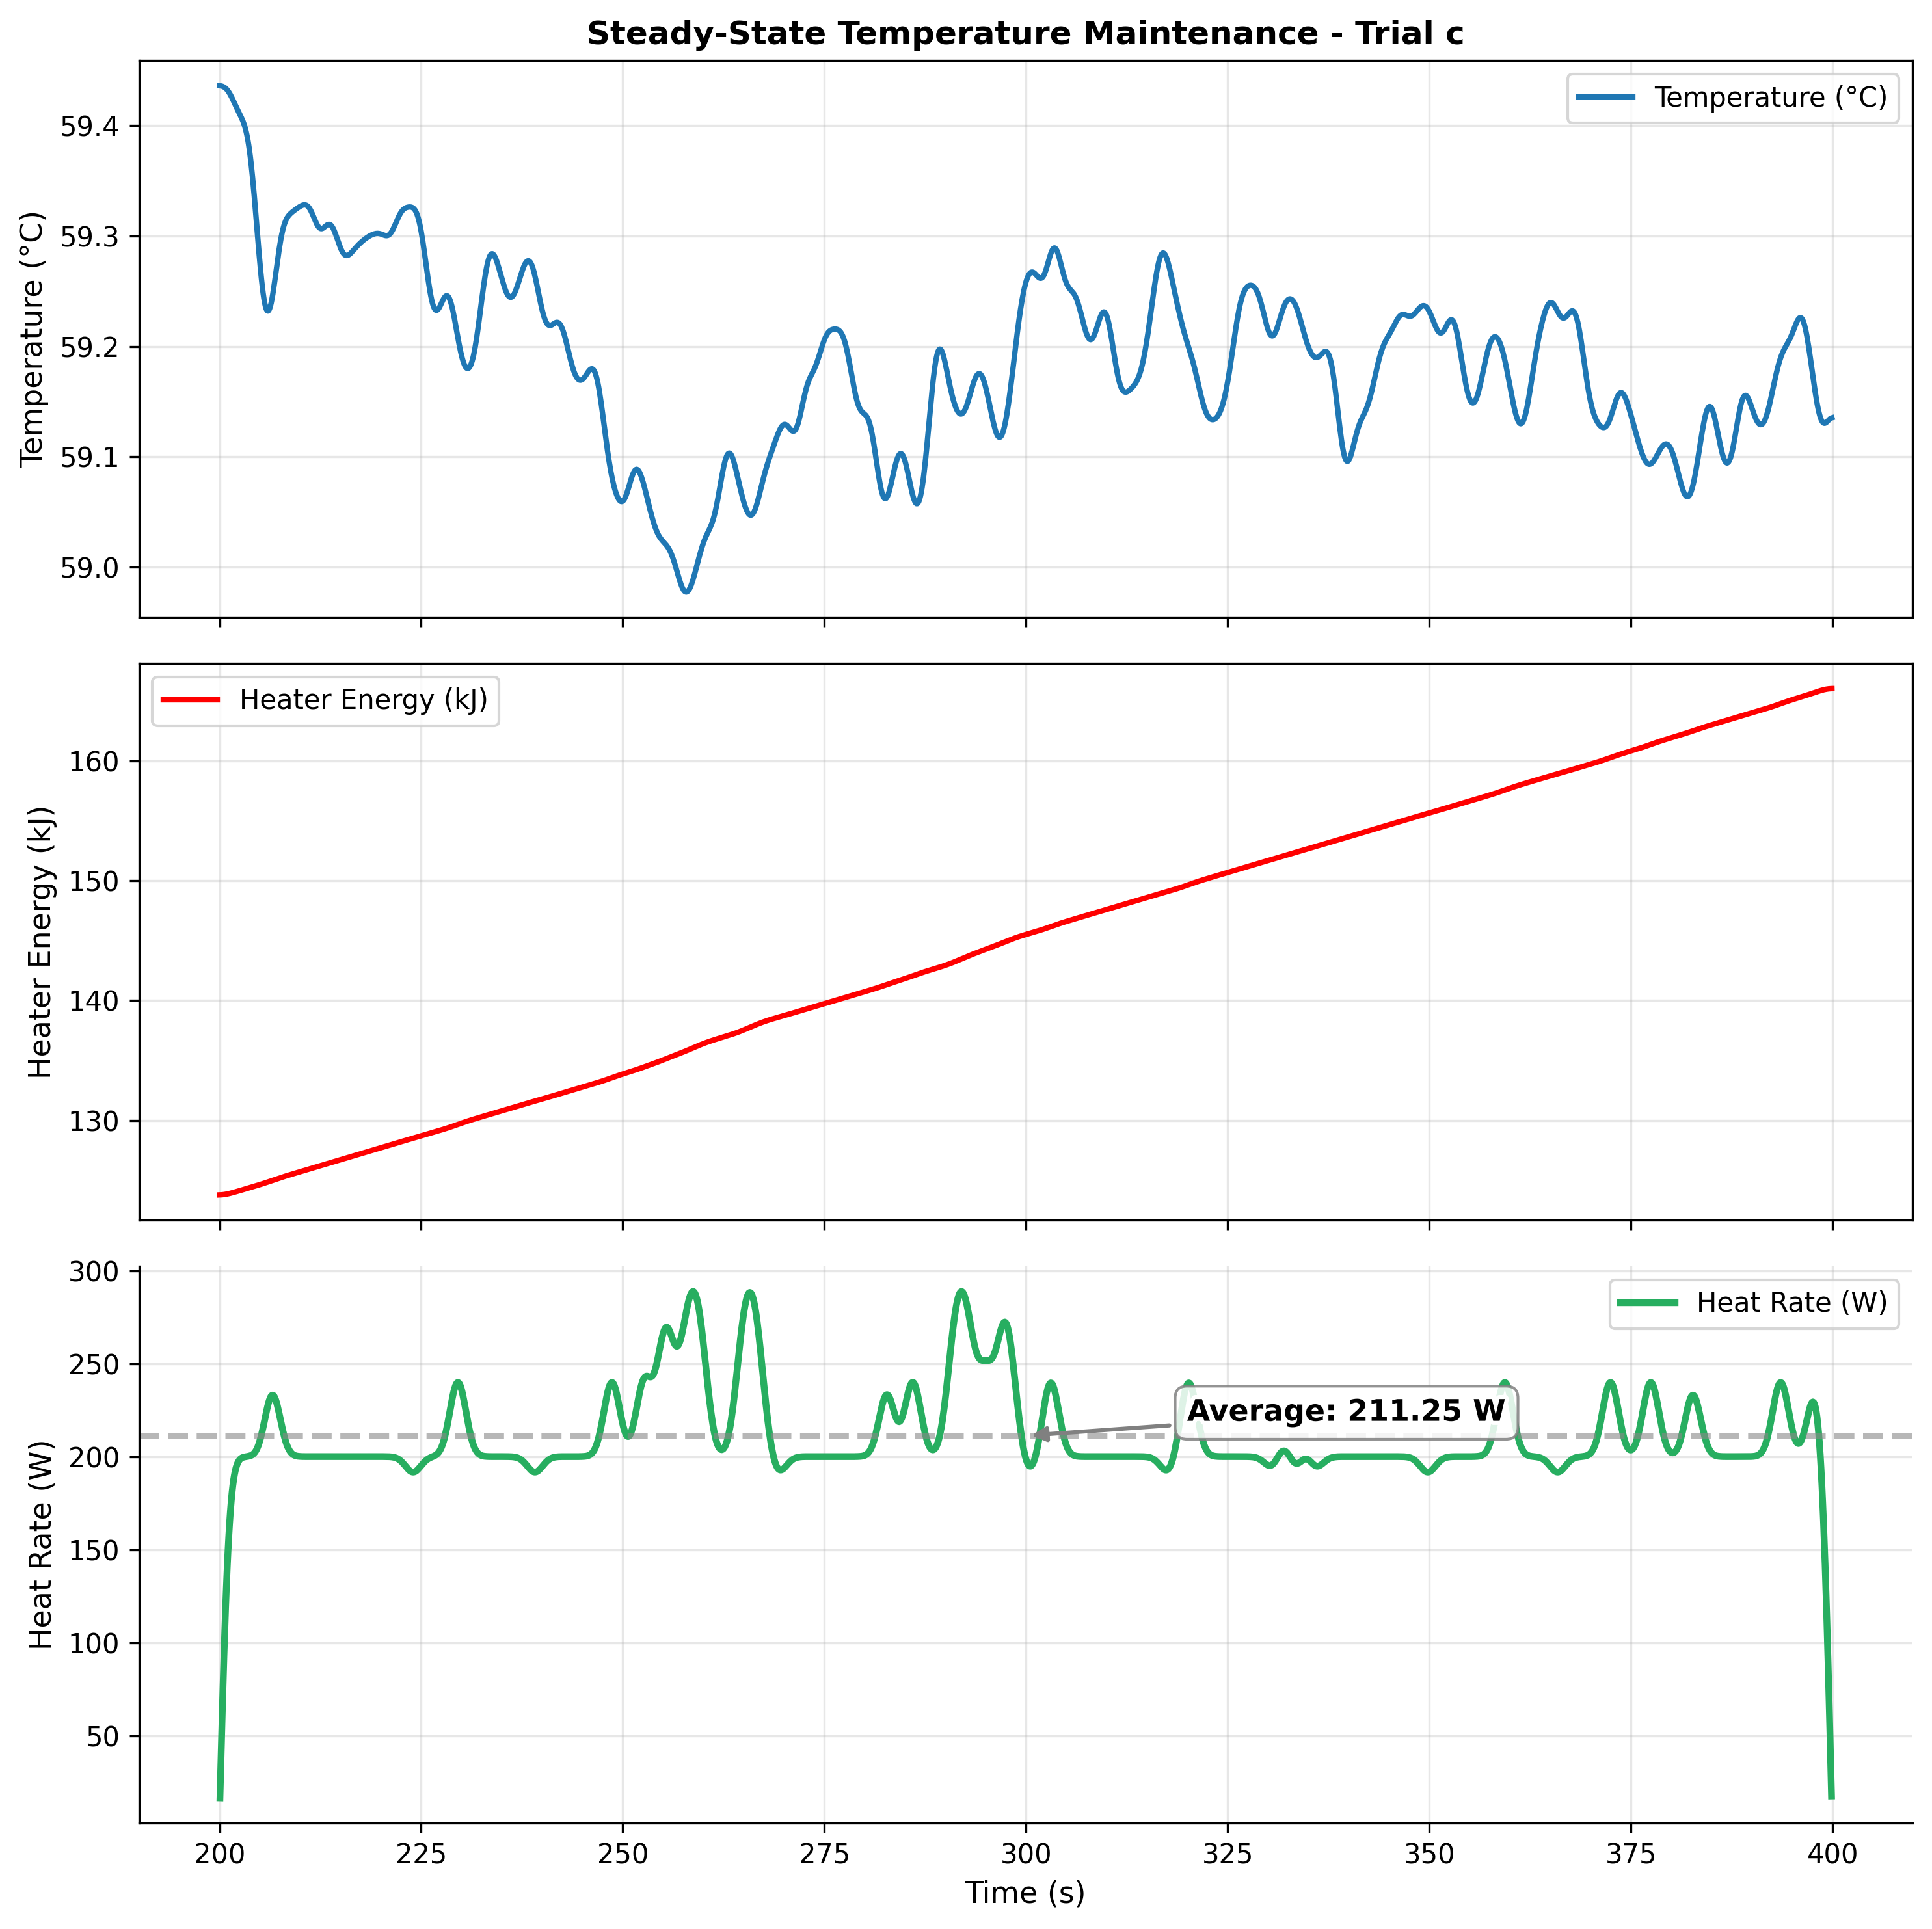
\includegraphics[width=0.85\textwidth]{graphs/part2_trial_c_heater_maintenance.png}
\caption{steady state plateau: Trial C.}
\end{figure}

\begin{figure}[H]
\centering
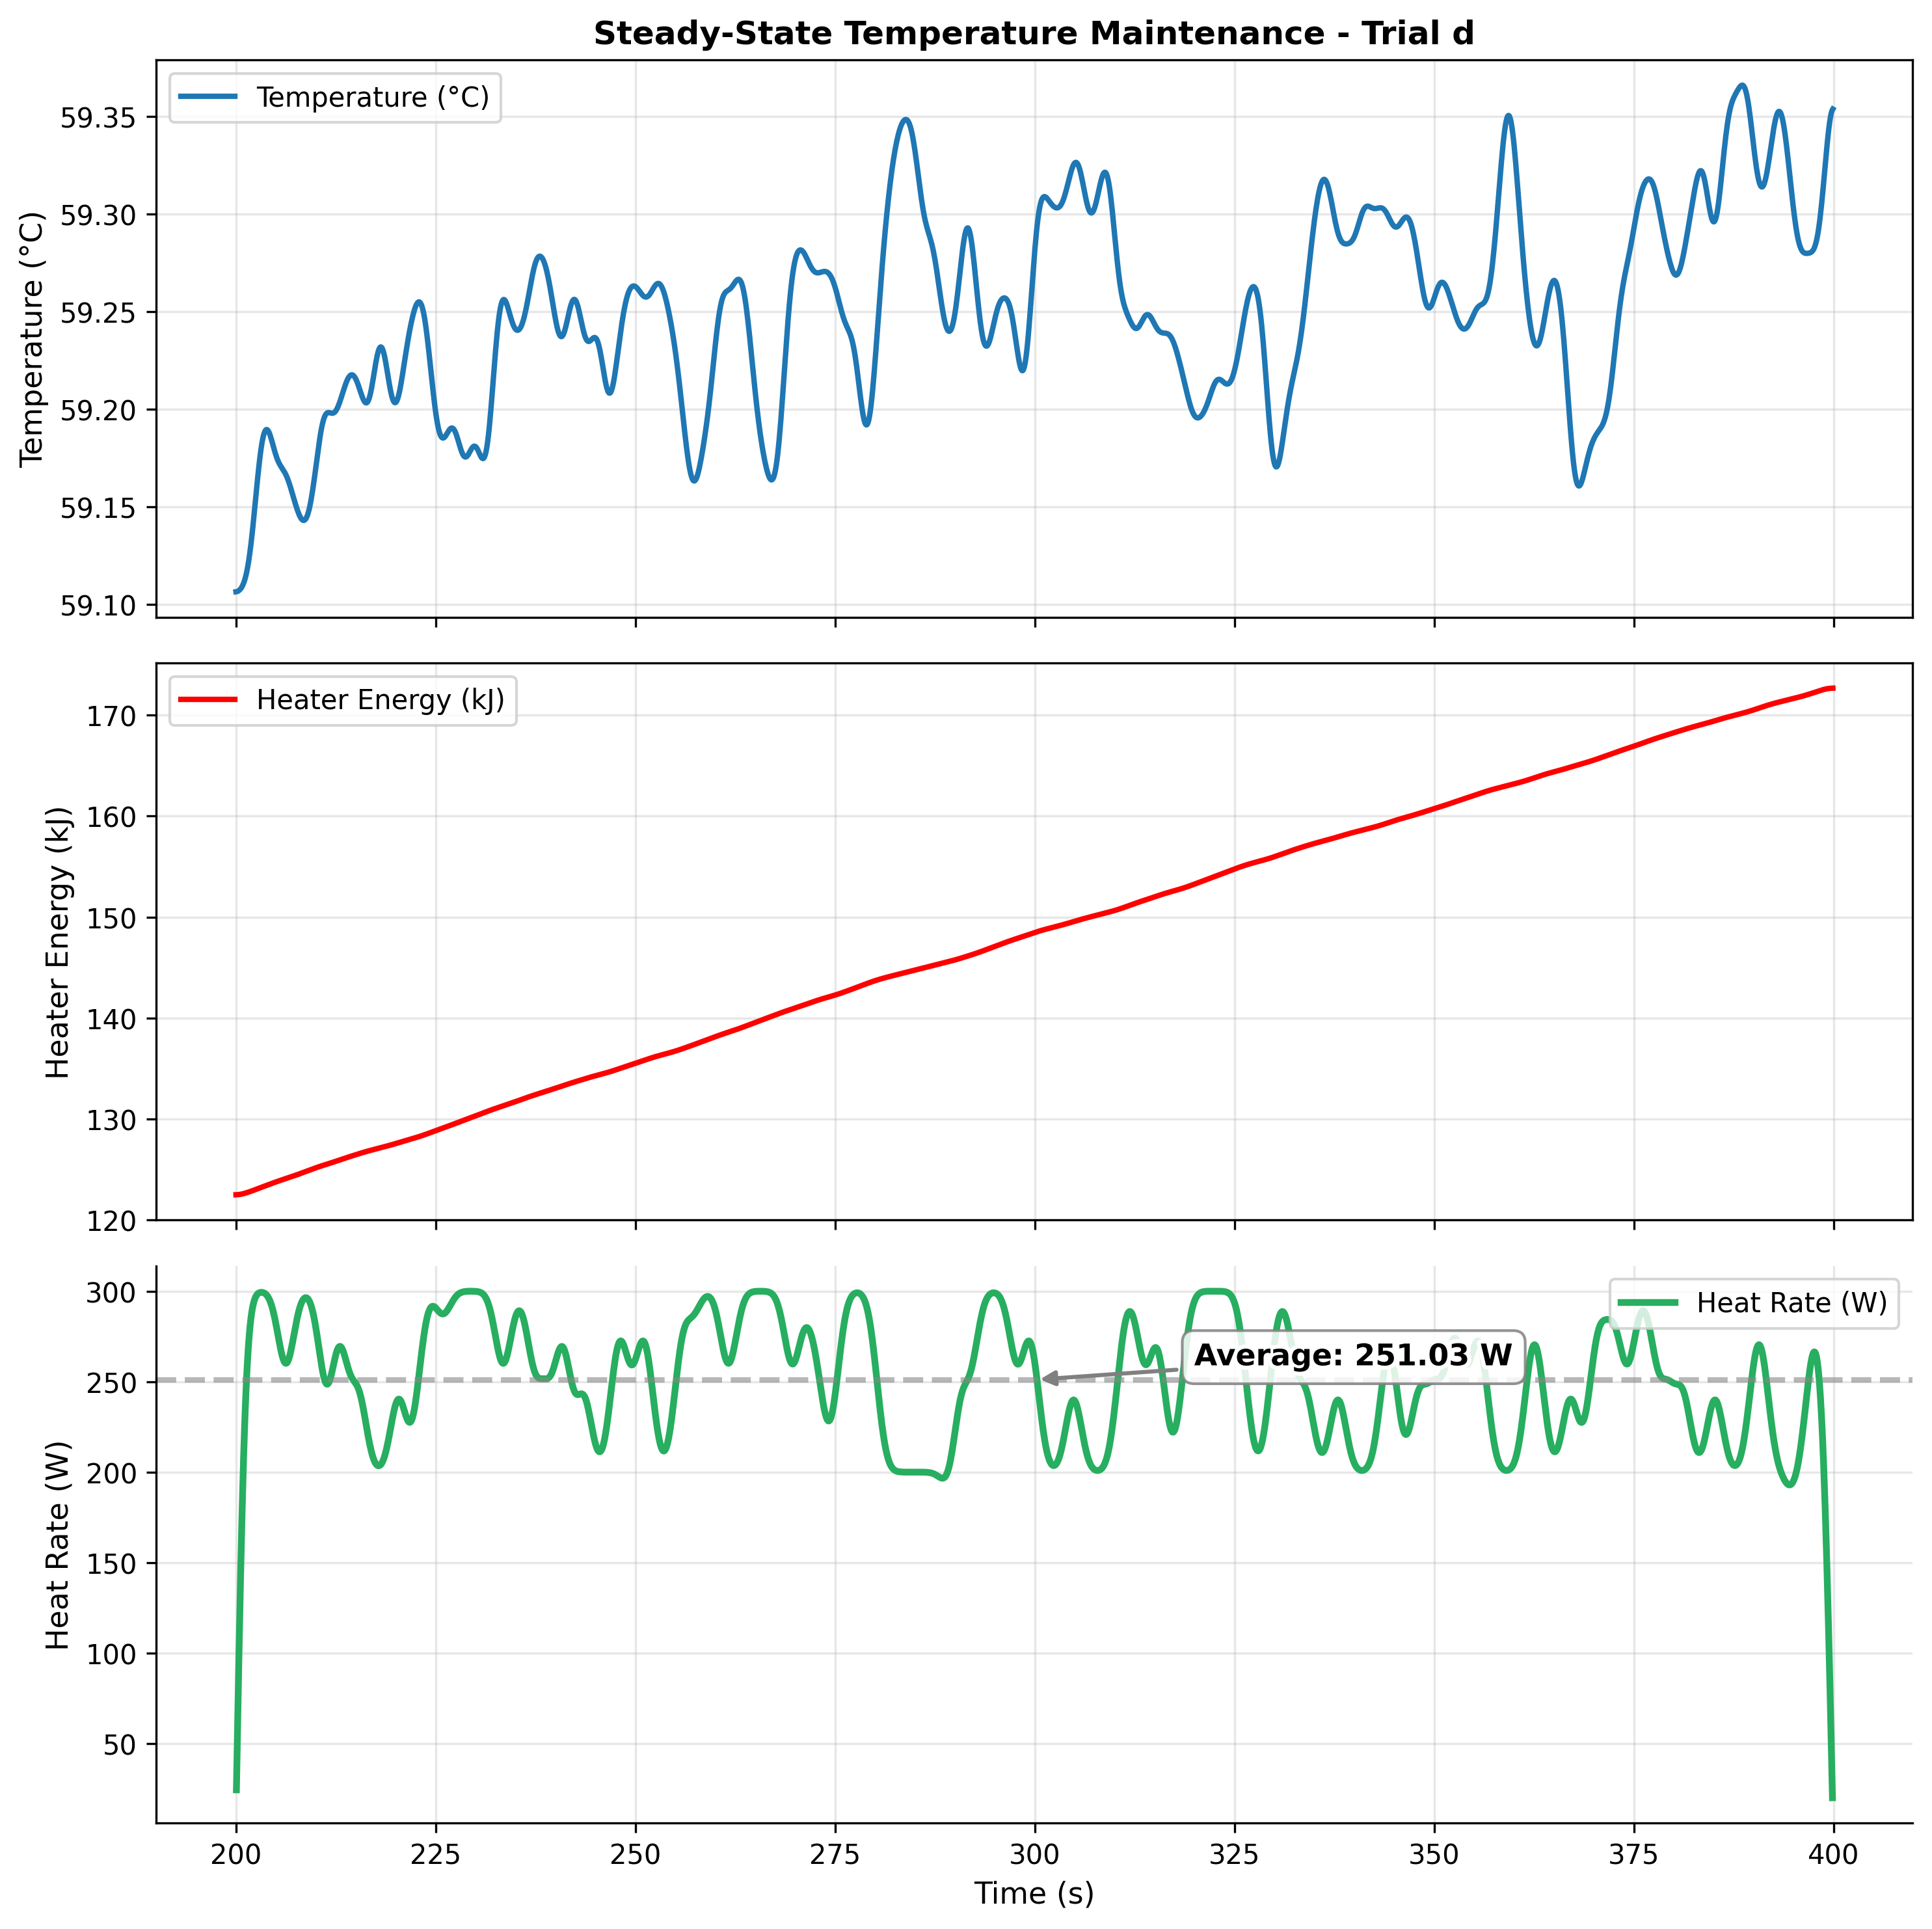
\includegraphics[width=0.85\textwidth]{graphs/part2_trial_d_heater_maintenance.png}
\caption{steady state plateau: Trial D.}
\end{figure}

\subsection*{B.4 Heat Loss Breakdown (Trials B, C, D)}

\begin{figure}[H]
\centering
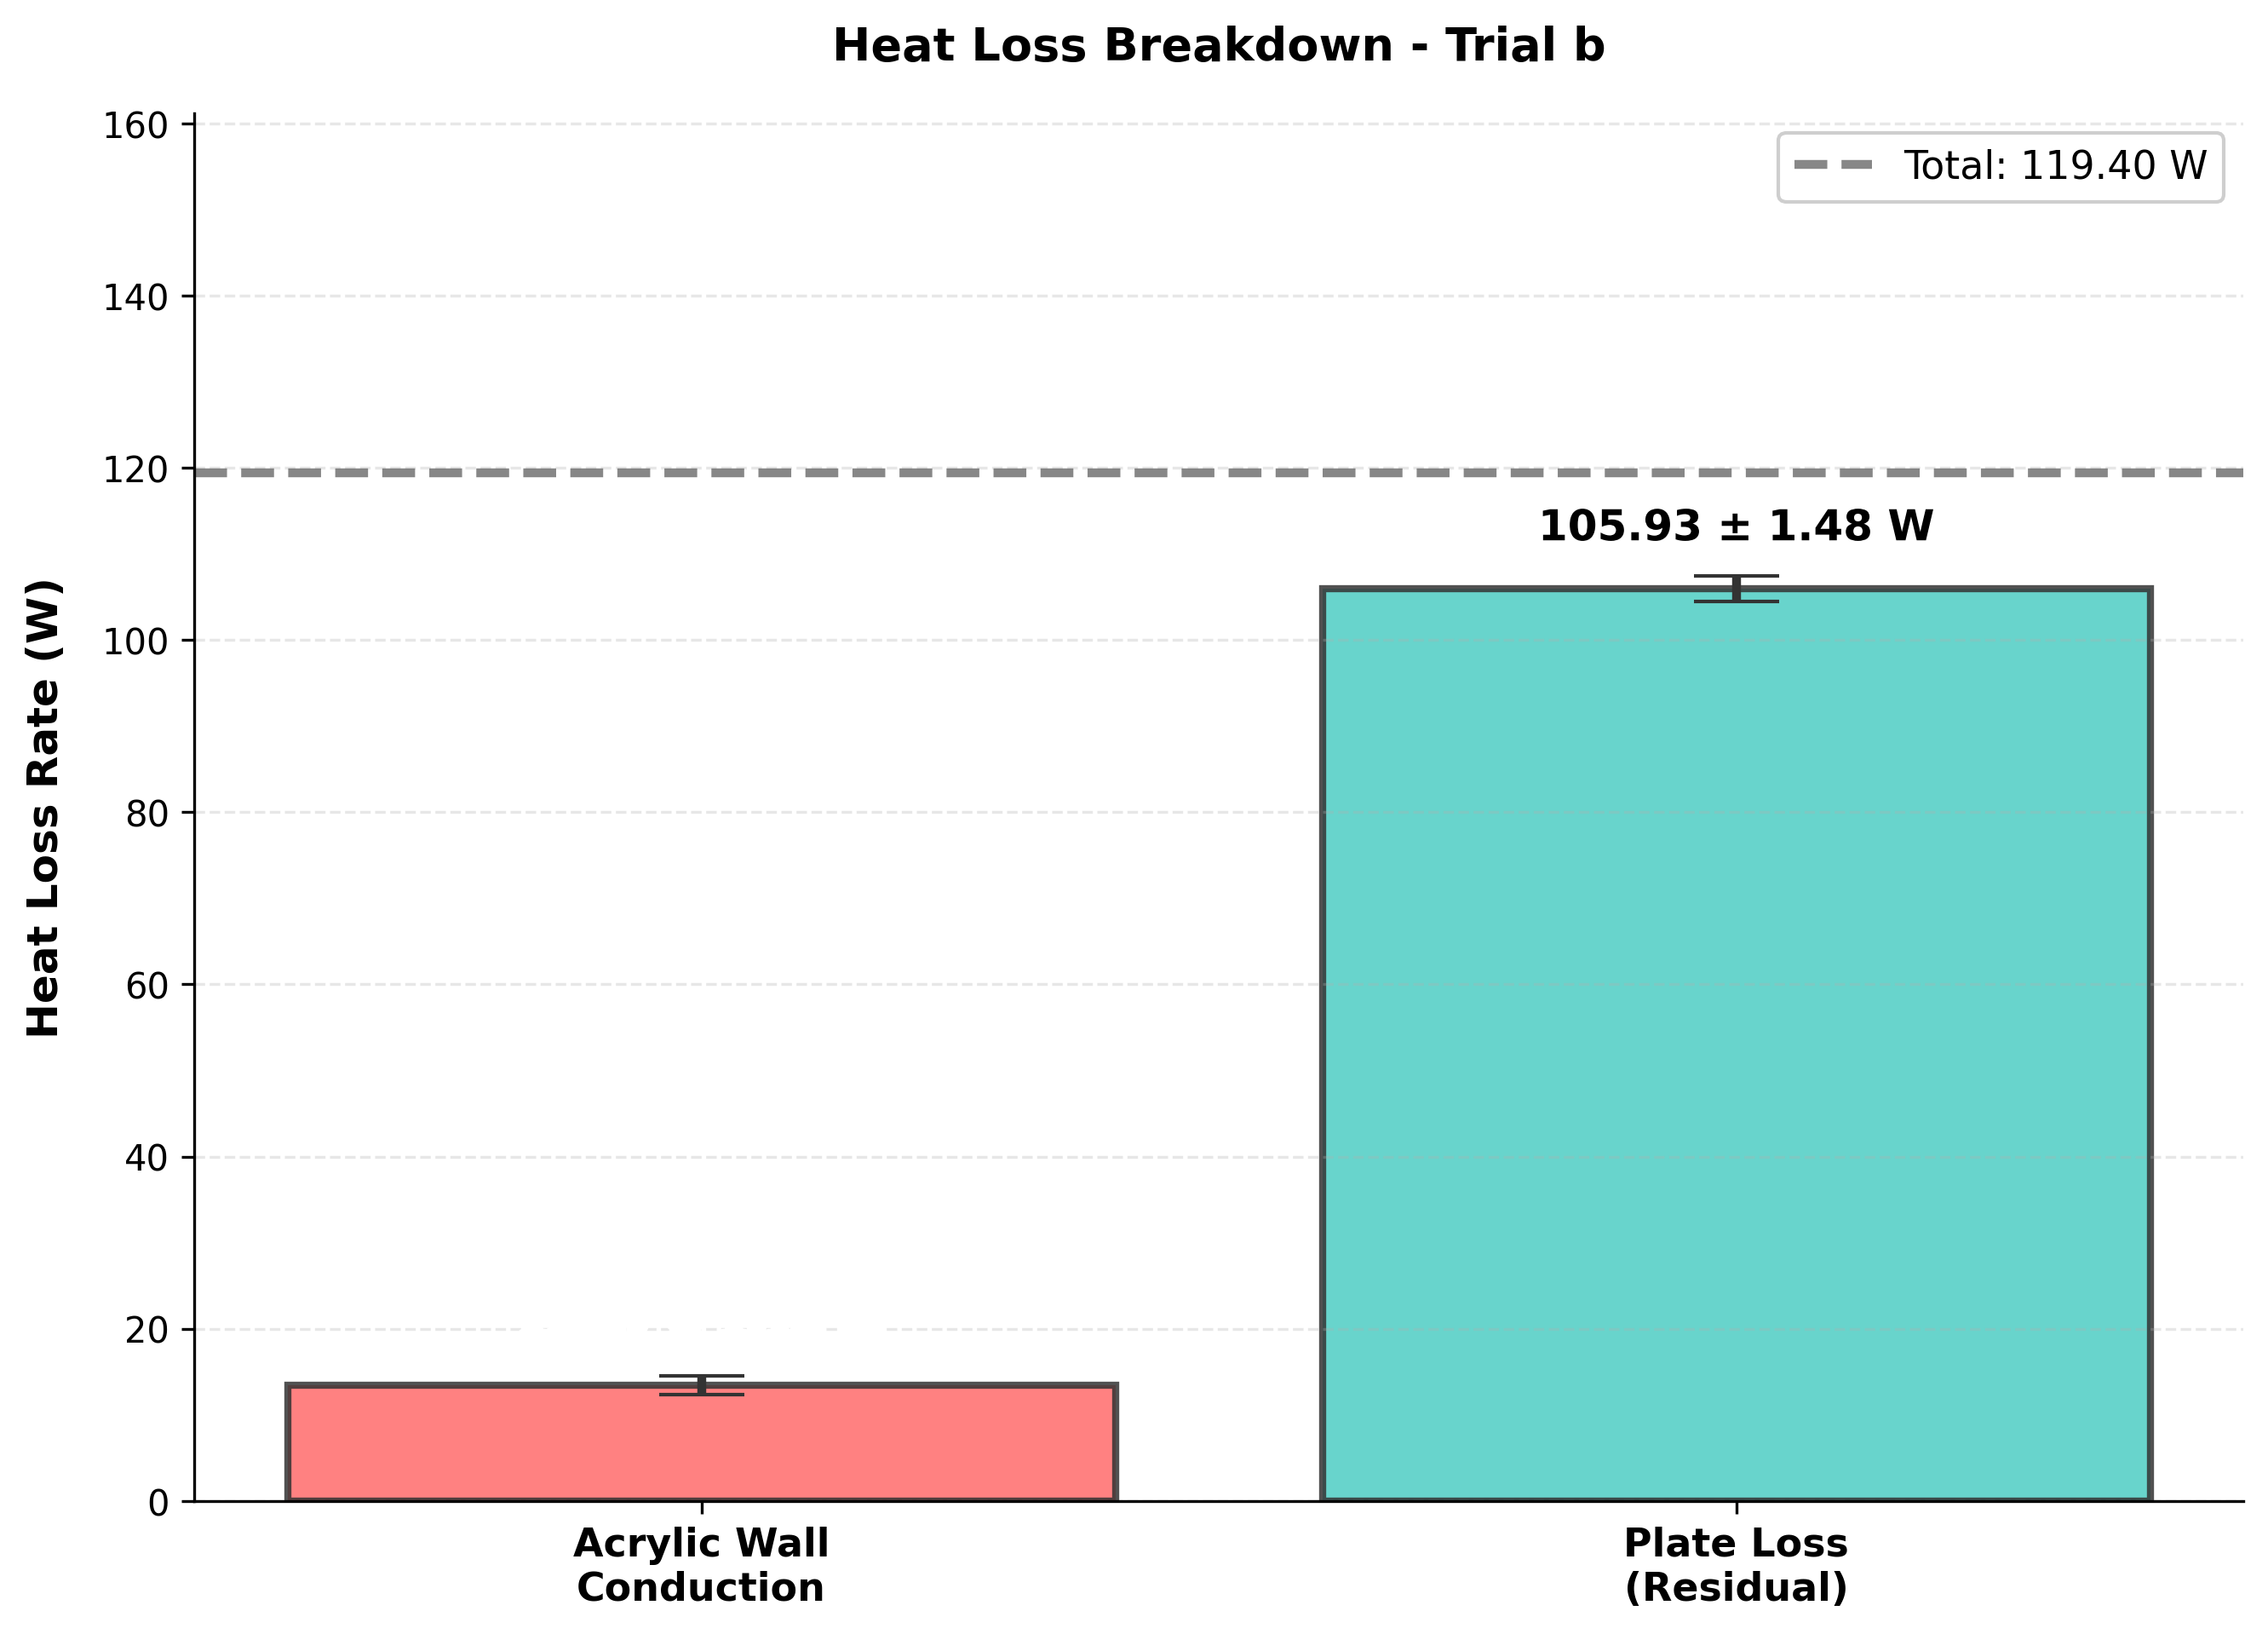
\includegraphics[width=0.85\textwidth]{graphs/part2_trial_b_loss_breakdown.png}
\caption{Heat loss breakdown (wall vs.\ plate): Trial B.}
\end{figure}

\begin{figure}[H]
\centering
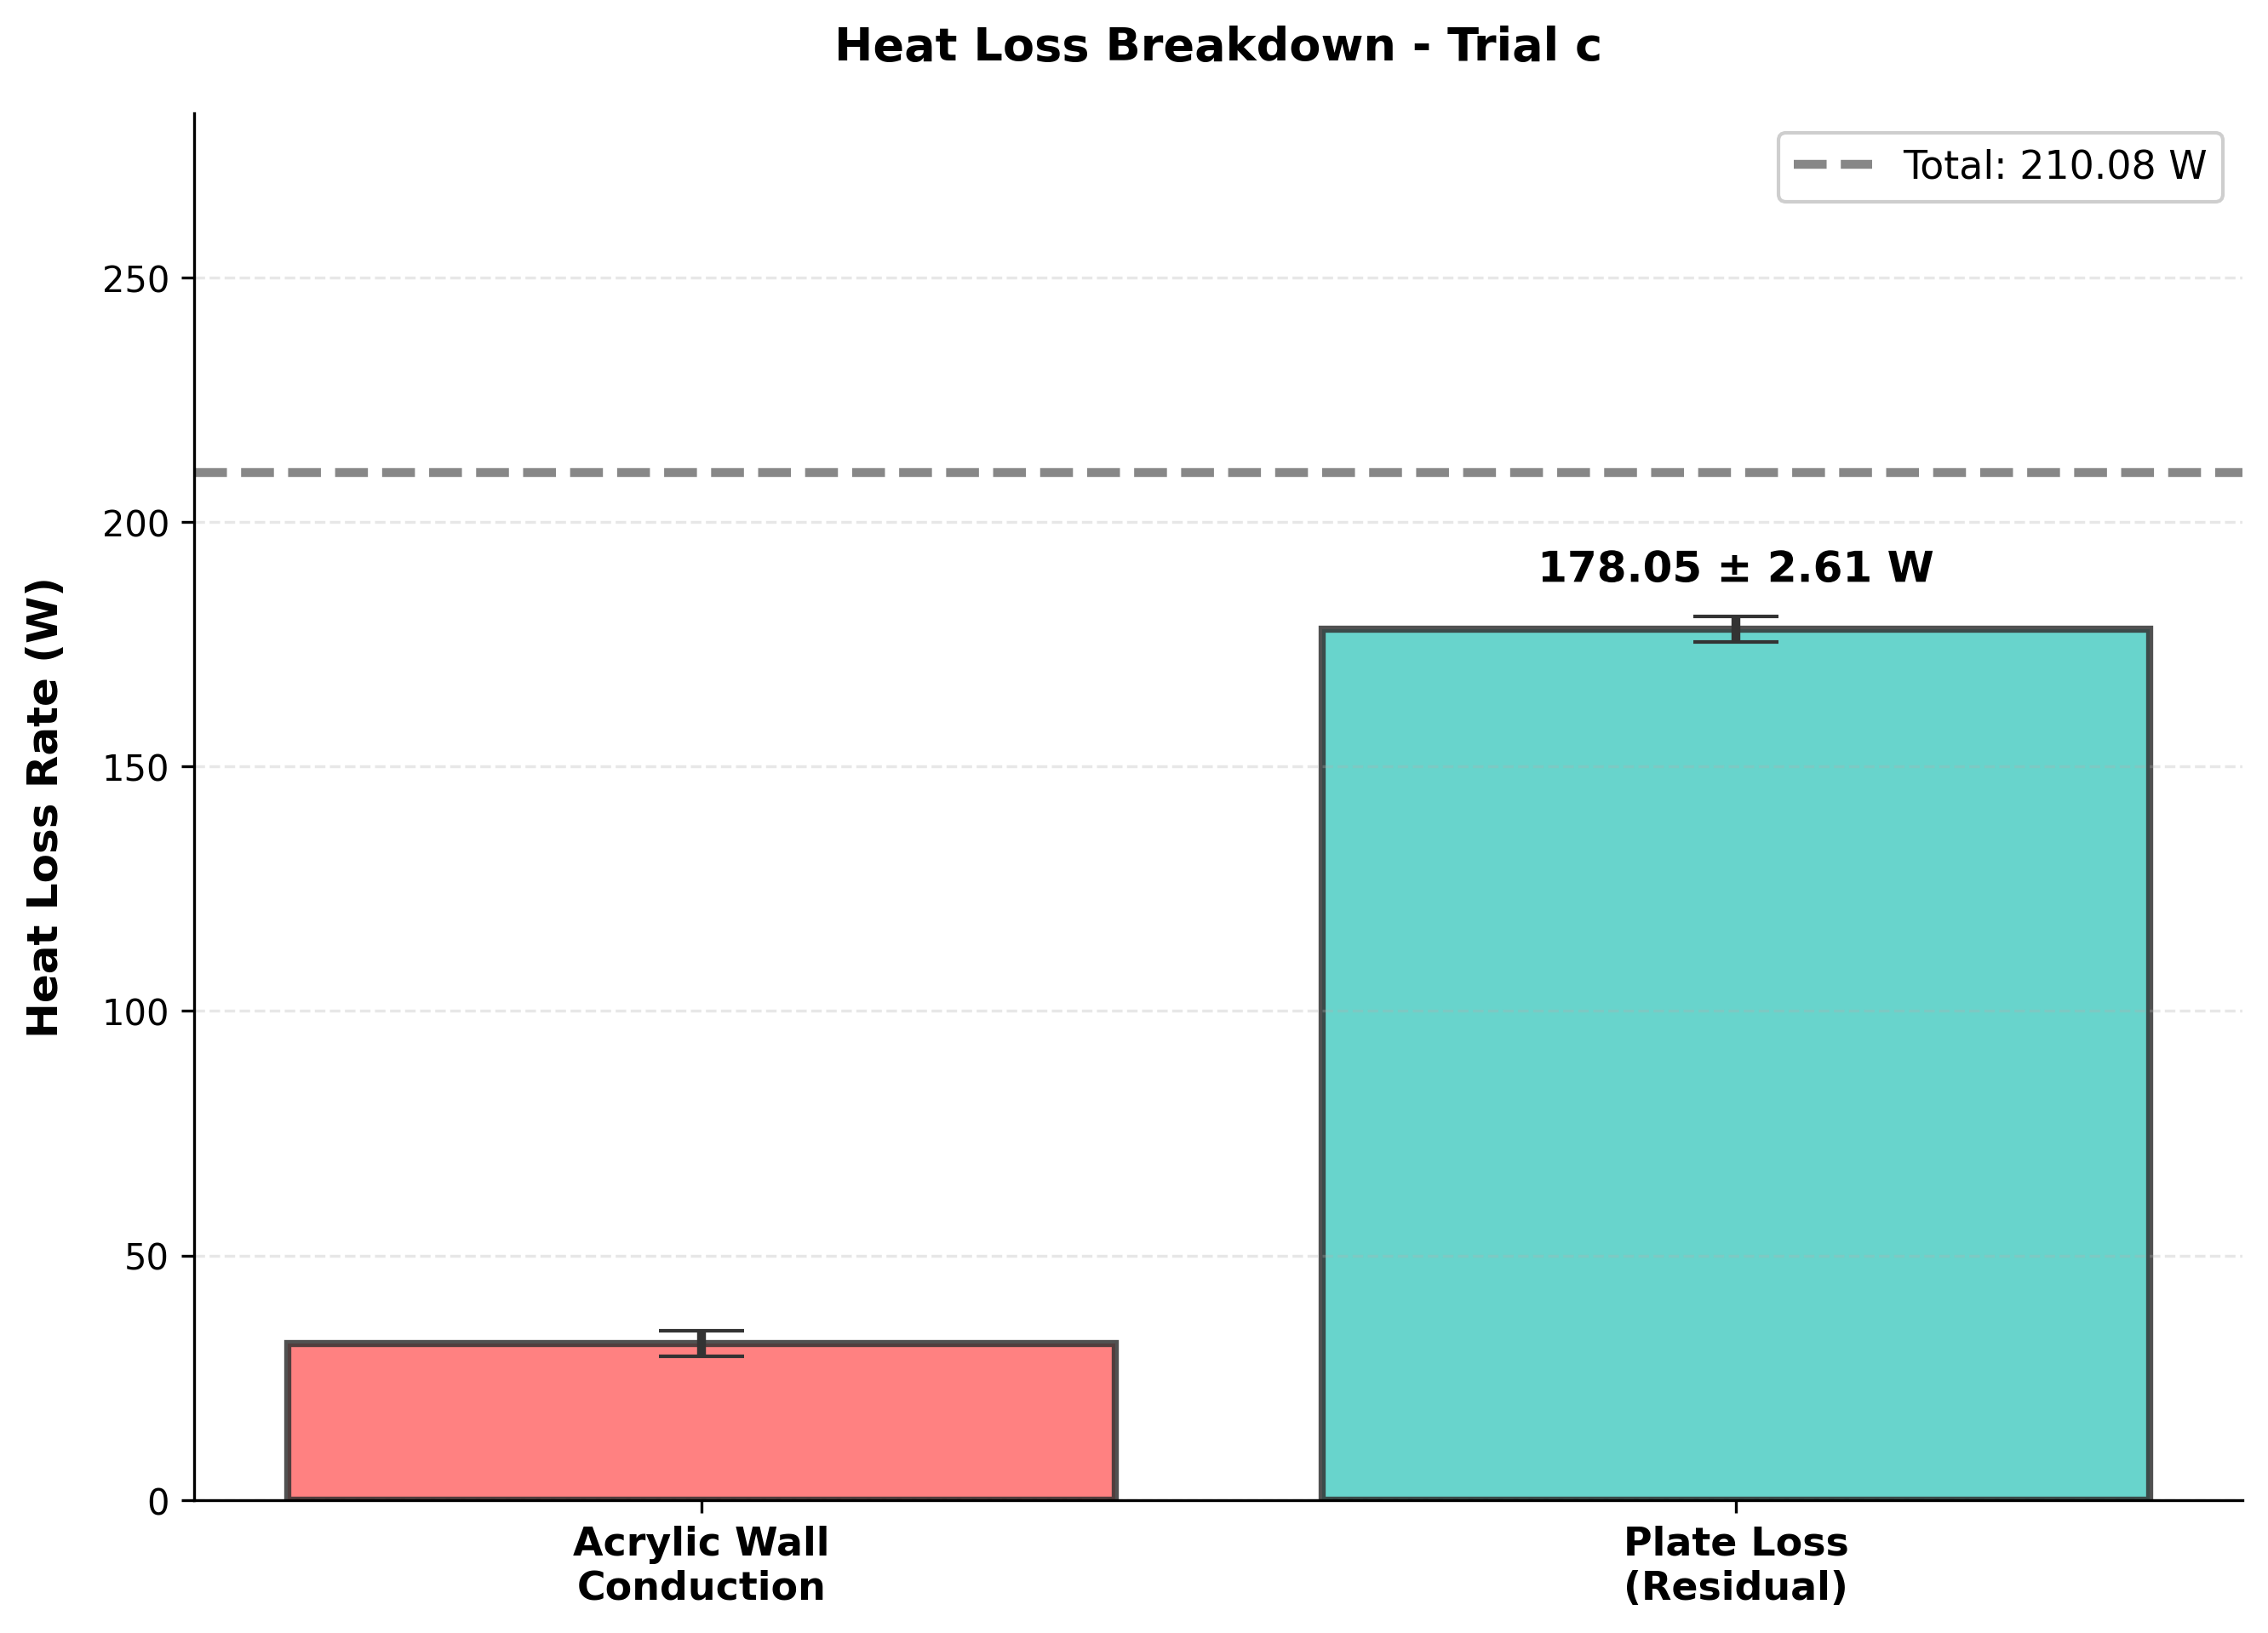
\includegraphics[width=0.85\textwidth]{graphs/part2_trial_c_loss_breakdown.png}
\caption{Heat loss breakdown (wall vs.\ plate): Trial C.}
\end{figure}

\begin{figure}[H]
\centering
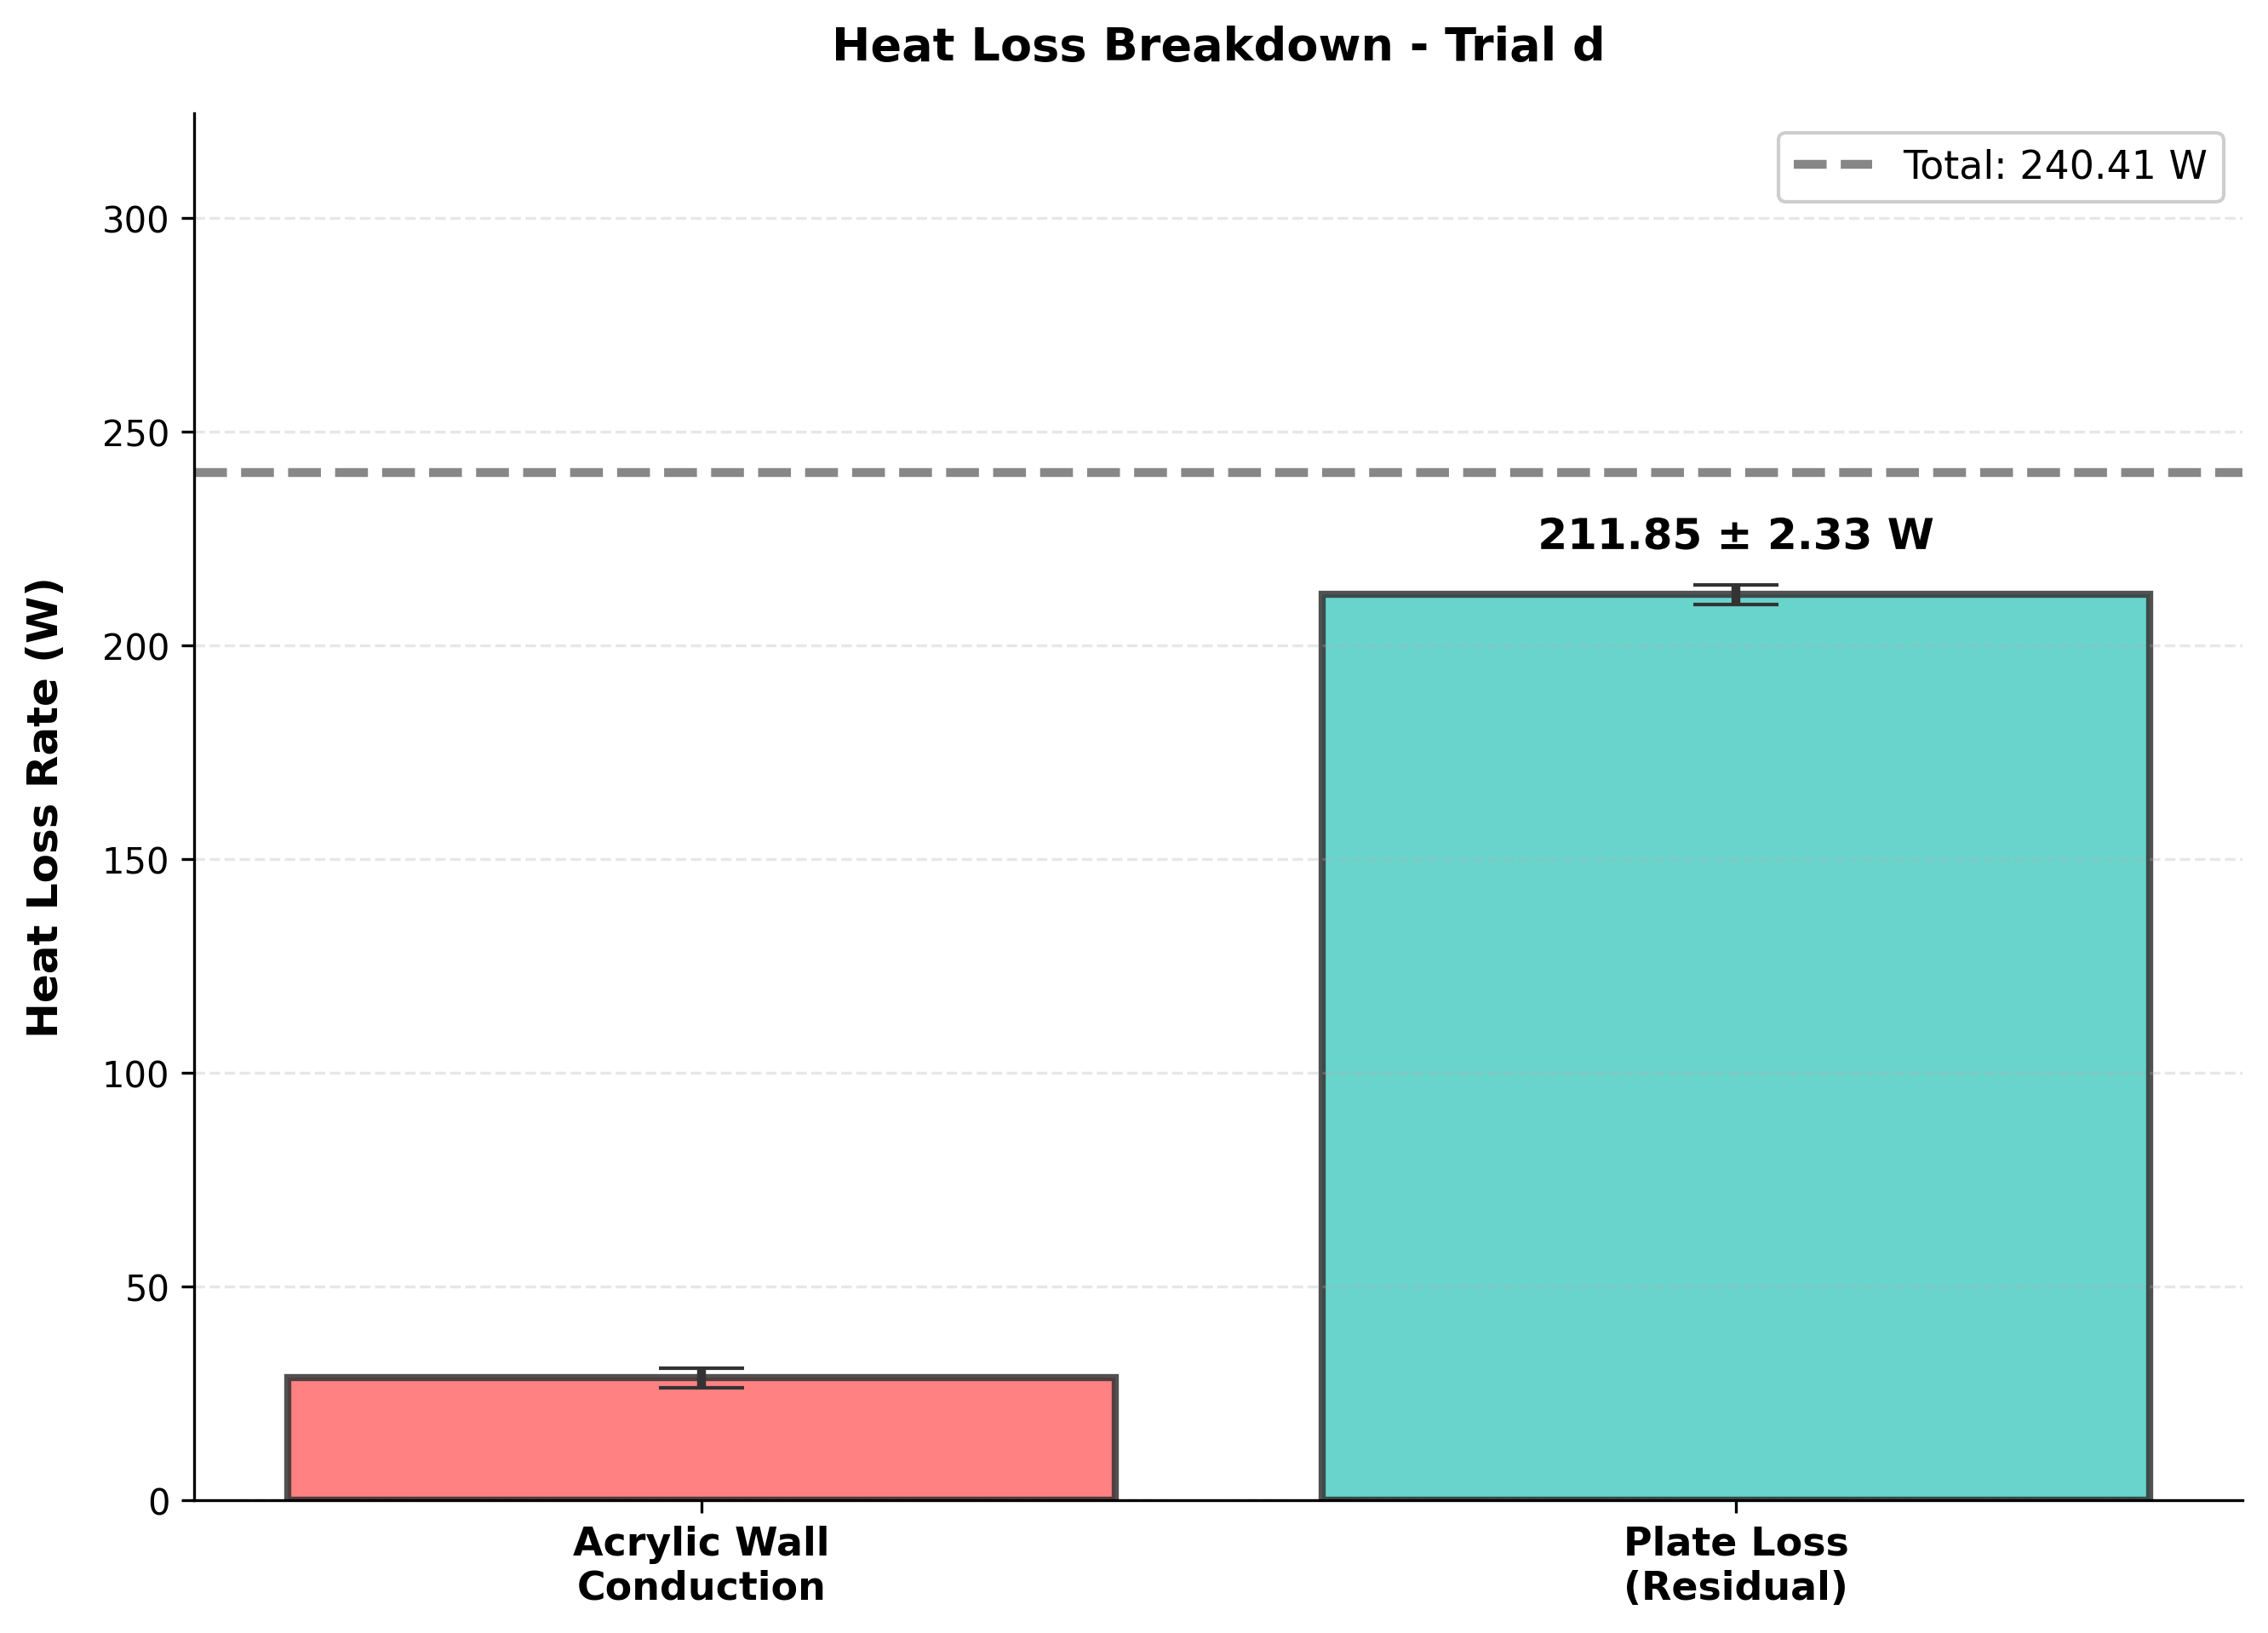
\includegraphics[width=0.85\textwidth]{graphs/part2_trial_d_loss_breakdown.png}
\caption{Heat loss breakdown (wall vs.\ plate): Trial D.}
\end{figure}

\end{document}
